% !TEX program = pdflatex
%
% Companion paper for the sparsegs / sparseGenSetCal framework.
%
% Every numeral in this file is a macro defined in numbers.tex, which
% experiments/make_numbers.py generates from the files the project produces.  A
% macro that reads (pending) marks a quantity whose input has not been computed
% yet; it is not a value to be trusted, and the draft is not finished while any
% of them remain.

\documentclass[11pt]{article}

\usepackage[T1]{fontenc}
\usepackage[utf8]{inputenc}
\usepackage[margin=2.4cm]{geometry}
\usepackage{amsmath,amssymb}
\usepackage{booktabs}
\usepackage{array}
\usepackage{graphicx}
\usepackage[numbers,sort&compress]{natbib}
\usepackage[colorlinks=true,allcolors=blue!55!black]{hyperref}
\usepackage{caption}
\usepackage{xcolor}
\usepackage{siunitx}
\usepackage{authblk}

\captionsetup{font=small,labelfont=bf}
\sisetup{detect-all}

% Generated by experiments/make_numbers.py -- do not edit.
%
% Every numeral the manuscript quotes is defined here, from the files
% the project produces.  A macro reading (pending) marks a quantity
% whose input is not on disk yet; it is not a value to be trusted.

\newcommand{\rankFrac}{0.05}
\newcommand{\gridARuns}{1,080}
% grid A, pooled: naive
\newcommand{\cellcorRate}{0.400}
\newcommand{\cellcorLo}{0.371}
\newcommand{\cellcorHi}{0.430}
\newcommand{\cellcorPct}{40.0}
\newcommand{\cellcorCalibrated}{no}
% grid A, pooled: permutation
\newcommand{\permutedRate}{0.397}
\newcommand{\permutedLo}{0.368}
\newcommand{\permutedHi}{0.427}
\newcommand{\permutedPct}{39.7}
\newcommand{\permutedCalibrated}{no}
% grid A, pooled: cutpoint_median
\newcommand{\cutmedRate}{0.337}
\newcommand{\cutmedLo}{0.309}
\newcommand{\cutmedHi}{0.366}
\newcommand{\cutmedPct}{33.7}
\newcommand{\cutmedCalibrated}{no}
% grid A, pooled: cutpoint_optimal
\newcommand{\cutoptRate}{0.556}
\newcommand{\cutoptLo}{0.527}
\newcommand{\cutoptHi}{0.586}
\newcommand{\cutoptPct}{55.6}
\newcommand{\cutoptCalibrated}{no}
% grid A, pooled: random
\newcommand{\randRate}{0.201}
\newcommand{\randLo}{0.178}
\newcommand{\randHi}{0.226}
\newcommand{\randPct}{20.1}
\newcommand{\randCalibrated}{no}
% grid A, pooled: expression
\newcommand{\exprRate}{0.068}
\newcommand{\exprLo}{0.054}
\newcommand{\exprHi}{0.084}
\newcommand{\exprPct}{6.8}
\newcommand{\exprCalibrated}{no}
% grid A, pooled: codetection
\newcommand{\codetRate}{0.094}
\newcommand{\codetLo}{0.078}
\newcommand{\codetHi}{0.113}
\newcommand{\codetPct}{9.4}
\newcommand{\codetCalibrated}{no}
\newcommand{\confLevels}{0, 0.3 and 0.6}
% confounding 0
\newcommand{\confAN}{360}
% programme-depth loading 0
\newcommand{\confALevel}{0}
% percentage points the outcome-chosen cutpoint costs over the median split at loading 0
\newcommand{\confACutCost}{23.1}
% confounding 0: naive
\newcommand{\confACellcor}{0.064}
% confounding 0: cutpoint_optimal
\newcommand{\confACutopt}{0.308}
% confounding 0: expression
\newcommand{\confAExpr}{0.069}
% confounding 0: codetection
\newcommand{\confACodet}{0.075}
% confounding 0.3
\newcommand{\confBN}{360}
% programme-depth loading 0.3
\newcommand{\confBLevel}{0.3}
% percentage points the outcome-chosen cutpoint costs over the median split at loading 0.3
\newcommand{\confBCutCost}{26.4}
% confounding 0.3: naive
\newcommand{\confBCellcor}{0.442}
% confounding 0.3: cutpoint_optimal
\newcommand{\confBCutopt}{0.586}
% confounding 0.3: expression
\newcommand{\confBExpr}{0.072}
% confounding 0.3: codetection
\newcommand{\confBCodet}{0.083}
% confounding 0.6
\newcommand{\confCN}{360}
% programme-depth loading 0.6
\newcommand{\confCLevel}{0.6}
% percentage points the outcome-chosen cutpoint costs over the median split at loading 0.6
\newcommand{\confCCutCost}{16.4}
% confounding 0.6: naive
\newcommand{\confCCellcor}{0.694}
% confounding 0.6: cutpoint_optimal
\newcommand{\confCCutopt}{0.775}
% confounding 0.6: expression
\newcommand{\confCExpr}{0.061}
% confounding 0.6: codetection
\newcommand{\confCCodet}{0.125}
\newcommand{\channelOpenN}{925}
% channel open: naive
\newcommand{\chanOpenCellcorRate}{0.395}
\newcommand{\chanOpenCellcorLo}{0.364}
\newcommand{\chanOpenCellcorHi}{0.426}
\newcommand{\chanOpenCellcorPct}{39.5}
% channel open: expression
\newcommand{\chanOpenExprRate}{0.065}
\newcommand{\chanOpenExprLo}{0.051}
\newcommand{\chanOpenExprHi}{0.083}
\newcommand{\chanOpenExprPct}{6.5}
% channel open: codetection
\newcommand{\chanOpenCodetRate}{0.085}
\newcommand{\chanOpenCodetLo}{0.069}
\newcommand{\chanOpenCodetHi}{0.105}
\newcommand{\chanOpenCodetPct}{8.5}
% channel open: random
\newcommand{\chanOpenRandRate}{0.188}
\newcommand{\chanOpenRandLo}{0.164}
\newcommand{\chanOpenRandHi}{0.215}
\newcommand{\chanOpenRandPct}{18.8}
\newcommand{\channelClosedN}{155}
% channel closed: naive
\newcommand{\chanClosedCellcorRate}{0.432}
\newcommand{\chanClosedCellcorLo}{0.357}
\newcommand{\chanClosedCellcorHi}{0.511}
\newcommand{\chanClosedCellcorPct}{43.2}
% channel closed: expression
\newcommand{\chanClosedExprRate}{0.084}
\newcommand{\chanClosedExprLo}{0.050}
\newcommand{\chanClosedExprHi}{0.138}
\newcommand{\chanClosedExprPct}{8.4}
% channel closed: codetection
\newcommand{\chanClosedCodetRate}{0.148}
\newcommand{\chanClosedCodetLo}{0.101}
\newcommand{\chanClosedCodetHi}{0.213}
\newcommand{\chanClosedCodetPct}{14.8}
% channel closed: random
\newcommand{\chanClosedRandRate}{0.277}
\newcommand{\chanClosedRandLo}{0.213}
\newcommand{\chanClosedRandHi}{0.353}
\newcommand{\chanClosedRandPct}{27.7}
% replicates per grid-A configuration
\newcommand{\gridAReplicates}{60}
% distinct grid-A configurations
\newcommand{\gridACells}{18}
% naive rejection in the lowest tie-break-share bin
\newcommand{\shareLowestRate}{0.583}
% naive rejection in the highest tie-break-share bin
\newcommand{\shareHighestRate}{0.283}
\newcommand{\shareLowestBin}{0.003}
\newcommand{\shareHighestBin}{0.703}
\newcommand{\shareMatchedLowest}{0.072}
\newcommand{\shareMatchedHighest}{0.083}
% naive-scale rejection in the lowest |implied rho| bin: naive
\newcommand{\impliedCellcorLowRate}{0.078}
\newcommand{\impliedCellcorLowLo}{0.047}
\newcommand{\impliedCellcorLowHi}{0.126}
% rejection in the highest |implied rho| bin: naive
\newcommand{\impliedCellcorHighRate}{1.000}
\newcommand{\impliedCellcorHighLo}{0.979}
\newcommand{\impliedCellcorHighHi}{1.000}
\newcommand{\impliedCellcorLowBin}{0.002}
\newcommand{\impliedCellcorHighBin}{0.297}
\newcommand{\impliedCellcorBins}{6}
% rejection in |implied rho| bin 1 of 6: naive
\newcommand{\impliedCellcorBinA}{0.078}
\newcommand{\impliedCellcorBinALo}{0.047}
\newcommand{\impliedCellcorBinAHi}{0.126}
% rejection in |implied rho| bin 2 of 6: naive
\newcommand{\impliedCellcorBinB}{0.044}
\newcommand{\impliedCellcorBinBLo}{0.023}
\newcommand{\impliedCellcorBinBHi}{0.085}
% rejection in |implied rho| bin 3 of 6: naive
\newcommand{\impliedCellcorBinC}{0.089}
\newcommand{\impliedCellcorBinCLo}{0.055}
\newcommand{\impliedCellcorBinCHi}{0.140}
% rejection in |implied rho| bin 4 of 6: naive
\newcommand{\impliedCellcorBinD}{0.356}
\newcommand{\impliedCellcorBinDLo}{0.289}
\newcommand{\impliedCellcorBinDHi}{0.428}
% rejection in |implied rho| bin 5 of 6: naive
\newcommand{\impliedCellcorBinE}{0.833}
\newcommand{\impliedCellcorBinELo}{0.772}
\newcommand{\impliedCellcorBinEHi}{0.881}
% rejection in |implied rho| bin 6 of 6: naive
\newcommand{\impliedCellcorBinF}{1.000}
\newcommand{\impliedCellcorBinFLo}{0.979}
\newcommand{\impliedCellcorBinFHi}{1.000}
% Cochran-Armitage trend in naive rejection across bins of implied
\newcommand{\impliedCellcorTrendZ}{+23.71}
% Cochran-Armitage P, naive against implied
\newcommand{\impliedCellcorTrendP}{\ensuremath{2.6\times10^{-124}}}
% Cochran-Armitage trend in naive rejection across bins of tie_break_share
\newcommand{\shareCellcorTrendZ}{-8.73}
% Cochran-Armitage P, naive against tie_break_share
\newcommand{\shareCellcorTrendP}{\ensuremath{2.6\times10^{-18}}}
% naive-scale rejection in the lowest |implied rho| bin: permutation
\newcommand{\impliedPermutedLowRate}{0.083}
\newcommand{\impliedPermutedLowLo}{0.051}
\newcommand{\impliedPermutedLowHi}{0.133}
% rejection in the highest |implied rho| bin: permutation
\newcommand{\impliedPermutedHighRate}{0.994}
\newcommand{\impliedPermutedHighLo}{0.969}
\newcommand{\impliedPermutedHighHi}{0.999}
\newcommand{\impliedPermutedLowBin}{0.002}
\newcommand{\impliedPermutedHighBin}{0.297}
\newcommand{\impliedPermutedBins}{6}
% rejection in |implied rho| bin 1 of 6: permutation
\newcommand{\impliedPermutedBinA}{0.083}
\newcommand{\impliedPermutedBinALo}{0.051}
\newcommand{\impliedPermutedBinAHi}{0.133}
% rejection in |implied rho| bin 2 of 6: permutation
\newcommand{\impliedPermutedBinB}{0.056}
\newcommand{\impliedPermutedBinBLo}{0.030}
\newcommand{\impliedPermutedBinBHi}{0.099}
% rejection in |implied rho| bin 3 of 6: permutation
\newcommand{\impliedPermutedBinC}{0.083}
\newcommand{\impliedPermutedBinCLo}{0.051}
\newcommand{\impliedPermutedBinCHi}{0.133}
% rejection in |implied rho| bin 4 of 6: permutation
\newcommand{\impliedPermutedBinD}{0.339}
\newcommand{\impliedPermutedBinDLo}{0.274}
\newcommand{\impliedPermutedBinDHi}{0.411}
% rejection in |implied rho| bin 5 of 6: permutation
\newcommand{\impliedPermutedBinE}{0.828}
\newcommand{\impliedPermutedBinELo}{0.766}
\newcommand{\impliedPermutedBinEHi}{0.876}
% rejection in |implied rho| bin 6 of 6: permutation
\newcommand{\impliedPermutedBinF}{0.994}
\newcommand{\impliedPermutedBinFLo}{0.969}
\newcommand{\impliedPermutedBinFHi}{0.999}
% Cochran-Armitage trend in permutation rejection across bins of implied
\newcommand{\impliedPermutedTrendZ}{+23.36}
% Cochran-Armitage P, permutation against implied
\newcommand{\impliedPermutedTrendP}{\ensuremath{1.1\times10^{-120}}}
% Cochran-Armitage trend in permutation rejection across bins of tie_break_share
\newcommand{\sharePermutedTrendZ}{-8.79}
% Cochran-Armitage P, permutation against tie_break_share
\newcommand{\sharePermutedTrendP}{\ensuremath{1.4\times10^{-18}}}
% naive-scale rejection in the lowest |implied rho| bin: cutpoint_median
\newcommand{\impliedCutmedLowRate}{0.100}
\newcommand{\impliedCutmedLowLo}{0.064}
\newcommand{\impliedCutmedLowHi}{0.153}
% rejection in the highest |implied rho| bin: cutpoint_median
\newcommand{\impliedCutmedHighRate}{0.917}
\newcommand{\impliedCutmedHighLo}{0.867}
\newcommand{\impliedCutmedHighHi}{0.949}
\newcommand{\impliedCutmedLowBin}{0.002}
\newcommand{\impliedCutmedHighBin}{0.297}
\newcommand{\impliedCutmedBins}{6}
% rejection in |implied rho| bin 1 of 6: cutpoint_median
\newcommand{\impliedCutmedBinA}{0.100}
\newcommand{\impliedCutmedBinALo}{0.064}
\newcommand{\impliedCutmedBinAHi}{0.153}
% rejection in |implied rho| bin 2 of 6: cutpoint_median
\newcommand{\impliedCutmedBinB}{0.050}
\newcommand{\impliedCutmedBinBLo}{0.027}
\newcommand{\impliedCutmedBinBHi}{0.092}
% rejection in |implied rho| bin 3 of 6: cutpoint_median
\newcommand{\impliedCutmedBinC}{0.089}
\newcommand{\impliedCutmedBinCLo}{0.055}
\newcommand{\impliedCutmedBinCHi}{0.140}
% rejection in |implied rho| bin 4 of 6: cutpoint_median
\newcommand{\impliedCutmedBinD}{0.311}
\newcommand{\impliedCutmedBinDLo}{0.248}
\newcommand{\impliedCutmedBinDHi}{0.382}
% rejection in |implied rho| bin 5 of 6: cutpoint_median
\newcommand{\impliedCutmedBinE}{0.556}
\newcommand{\impliedCutmedBinELo}{0.483}
\newcommand{\impliedCutmedBinEHi}{0.626}
% rejection in |implied rho| bin 6 of 6: cutpoint_median
\newcommand{\impliedCutmedBinF}{0.917}
\newcommand{\impliedCutmedBinFLo}{0.867}
\newcommand{\impliedCutmedBinFHi}{0.949}
% Cochran-Armitage trend in cutpoint_median rejection across bins of implied
\newcommand{\impliedCutmedTrendZ}{+19.75}
% Cochran-Armitage P, cutpoint_median against implied
\newcommand{\impliedCutmedTrendP}{\ensuremath{7.8\times10^{-87}}}
% Cochran-Armitage trend in cutpoint_median rejection across bins of tie_break_share
\newcommand{\shareCutmedTrendZ}{-7.39}
% Cochran-Armitage P, cutpoint_median against tie_break_share
\newcommand{\shareCutmedTrendP}{\ensuremath{1.5\times10^{-13}}}
% naive-scale rejection in the lowest |implied rho| bin: cutpoint_optimal
\newcommand{\impliedCutoptLowRate}{0.294}
\newcommand{\impliedCutoptLowLo}{0.233}
\newcommand{\impliedCutoptLowHi}{0.365}
% rejection in the highest |implied rho| bin: cutpoint_optimal
\newcommand{\impliedCutoptHighRate}{0.994}
\newcommand{\impliedCutoptHighLo}{0.969}
\newcommand{\impliedCutoptHighHi}{0.999}
\newcommand{\impliedCutoptLowBin}{0.002}
\newcommand{\impliedCutoptHighBin}{0.297}
\newcommand{\impliedCutoptBins}{6}
% rejection in |implied rho| bin 1 of 6: cutpoint_optimal
\newcommand{\impliedCutoptBinA}{0.294}
\newcommand{\impliedCutoptBinALo}{0.233}
\newcommand{\impliedCutoptBinAHi}{0.365}
% rejection in |implied rho| bin 2 of 6: cutpoint_optimal
\newcommand{\impliedCutoptBinB}{0.300}
\newcommand{\impliedCutoptBinBLo}{0.238}
\newcommand{\impliedCutoptBinBHi}{0.371}
% rejection in |implied rho| bin 3 of 6: cutpoint_optimal
\newcommand{\impliedCutoptBinC}{0.306}
\newcommand{\impliedCutoptBinCLo}{0.243}
\newcommand{\impliedCutoptBinCHi}{0.376}
% rejection in |implied rho| bin 4 of 6: cutpoint_optimal
\newcommand{\impliedCutoptBinD}{0.589}
\newcommand{\impliedCutoptBinDLo}{0.516}
\newcommand{\impliedCutoptBinDHi}{0.658}
% rejection in |implied rho| bin 5 of 6: cutpoint_optimal
\newcommand{\impliedCutoptBinE}{0.856}
\newcommand{\impliedCutoptBinELo}{0.797}
\newcommand{\impliedCutoptBinEHi}{0.899}
% rejection in |implied rho| bin 6 of 6: cutpoint_optimal
\newcommand{\impliedCutoptBinF}{0.994}
\newcommand{\impliedCutoptBinFLo}{0.969}
\newcommand{\impliedCutoptBinFHi}{0.999}
% Cochran-Armitage trend in cutpoint_optimal rejection across bins of implied
\newcommand{\impliedCutoptTrendZ}{+17.59}
% Cochran-Armitage P, cutpoint_optimal against implied
\newcommand{\impliedCutoptTrendP}{\ensuremath{2.9\times10^{-69}}}
% Cochran-Armitage trend in cutpoint_optimal rejection across bins of tie_break_share
\newcommand{\shareCutoptTrendZ}{-9.63}
% Cochran-Armitage P, cutpoint_optimal against tie_break_share
\newcommand{\shareCutoptTrendP}{\ensuremath{6.0\times10^{-22}}}
% naive-scale rejection in the lowest |implied rho| bin: random
\newcommand{\impliedRandLowRate}{0.072}
\newcommand{\impliedRandLowLo}{0.043}
\newcommand{\impliedRandLowHi}{0.120}
% rejection in the highest |implied rho| bin: random
\newcommand{\impliedRandHighRate}{0.717}
\newcommand{\impliedRandHighLo}{0.647}
\newcommand{\impliedRandHighHi}{0.777}
\newcommand{\impliedRandLowBin}{0.002}
\newcommand{\impliedRandHighBin}{0.297}
\newcommand{\impliedRandBins}{6}
% rejection in |implied rho| bin 1 of 6: random
\newcommand{\impliedRandBinA}{0.072}
\newcommand{\impliedRandBinALo}{0.043}
\newcommand{\impliedRandBinAHi}{0.120}
% rejection in |implied rho| bin 2 of 6: random
\newcommand{\impliedRandBinB}{0.050}
\newcommand{\impliedRandBinBLo}{0.027}
\newcommand{\impliedRandBinBHi}{0.092}
% rejection in |implied rho| bin 3 of 6: random
\newcommand{\impliedRandBinC}{0.022}
\newcommand{\impliedRandBinCLo}{0.009}
\newcommand{\impliedRandBinCHi}{0.056}
% rejection in |implied rho| bin 4 of 6: random
\newcommand{\impliedRandBinD}{0.061}
\newcommand{\impliedRandBinDLo}{0.034}
\newcommand{\impliedRandBinDHi}{0.106}
% rejection in |implied rho| bin 5 of 6: random
\newcommand{\impliedRandBinE}{0.283}
\newcommand{\impliedRandBinELo}{0.223}
\newcommand{\impliedRandBinEHi}{0.353}
% rejection in |implied rho| bin 6 of 6: random
\newcommand{\impliedRandBinF}{0.717}
\newcommand{\impliedRandBinFLo}{0.647}
\newcommand{\impliedRandBinFHi}{0.777}
% Cochran-Armitage trend in random rejection across bins of implied
\newcommand{\impliedRandTrendZ}{+15.85}
% Cochran-Armitage P, random against implied
\newcommand{\impliedRandTrendP}{\ensuremath{1.4\times10^{-56}}}
% Cochran-Armitage trend in random rejection across bins of tie_break_share
\newcommand{\shareRandTrendZ}{-11.58}
% Cochran-Armitage P, random against tie_break_share
\newcommand{\shareRandTrendP}{\ensuremath{5.0\times10^{-31}}}
% naive-scale rejection in the lowest |implied rho| bin: expression
\newcommand{\impliedExprLowRate}{0.089}
\newcommand{\impliedExprLowLo}{0.055}
\newcommand{\impliedExprLowHi}{0.140}
% rejection in the highest |implied rho| bin: expression
\newcommand{\impliedExprHighRate}{0.083}
\newcommand{\impliedExprHighLo}{0.051}
\newcommand{\impliedExprHighHi}{0.133}
\newcommand{\impliedExprLowBin}{0.002}
\newcommand{\impliedExprHighBin}{0.297}
\newcommand{\impliedExprBins}{6}
% rejection in |implied rho| bin 1 of 6: expression
\newcommand{\impliedExprBinA}{0.089}
\newcommand{\impliedExprBinALo}{0.055}
\newcommand{\impliedExprBinAHi}{0.140}
% rejection in |implied rho| bin 2 of 6: expression
\newcommand{\impliedExprBinB}{0.050}
\newcommand{\impliedExprBinBLo}{0.027}
\newcommand{\impliedExprBinBHi}{0.092}
% rejection in |implied rho| bin 3 of 6: expression
\newcommand{\impliedExprBinC}{0.067}
\newcommand{\impliedExprBinCLo}{0.039}
\newcommand{\impliedExprBinCHi}{0.113}
% rejection in |implied rho| bin 4 of 6: expression
\newcommand{\impliedExprBinD}{0.028}
\newcommand{\impliedExprBinDLo}{0.012}
\newcommand{\impliedExprBinDHi}{0.063}
% rejection in |implied rho| bin 5 of 6: expression
\newcommand{\impliedExprBinE}{0.089}
\newcommand{\impliedExprBinELo}{0.055}
\newcommand{\impliedExprBinEHi}{0.140}
% rejection in |implied rho| bin 6 of 6: expression
\newcommand{\impliedExprBinF}{0.083}
\newcommand{\impliedExprBinFLo}{0.051}
\newcommand{\impliedExprBinFHi}{0.133}
% Cochran-Armitage trend in expression rejection across bins of implied
\newcommand{\impliedExprTrendZ}{+0.32}
% Cochran-Armitage P, expression against implied
\newcommand{\impliedExprTrendP}{\ensuremath{7.5\times10^{-1}}}
% Cochran-Armitage trend in expression rejection across bins of tie_break_share
\newcommand{\shareExprTrendZ}{+0.25}
% Cochran-Armitage P, expression against tie_break_share
\newcommand{\shareExprTrendP}{\ensuremath{8.0\times10^{-1}}}
% naive-scale rejection in the lowest |implied rho| bin: codetection
\newcommand{\impliedCodetLowRate}{0.094}
\newcommand{\impliedCodetLowLo}{0.060}
\newcommand{\impliedCodetLowHi}{0.146}
% rejection in the highest |implied rho| bin: codetection
\newcommand{\impliedCodetHighRate}{0.183}
\newcommand{\impliedCodetHighLo}{0.134}
\newcommand{\impliedCodetHighHi}{0.246}
\newcommand{\impliedCodetLowBin}{0.002}
\newcommand{\impliedCodetHighBin}{0.297}
\newcommand{\impliedCodetBins}{6}
% rejection in |implied rho| bin 1 of 6: codetection
\newcommand{\impliedCodetBinA}{0.094}
\newcommand{\impliedCodetBinALo}{0.060}
\newcommand{\impliedCodetBinAHi}{0.146}
% rejection in |implied rho| bin 2 of 6: codetection
\newcommand{\impliedCodetBinB}{0.061}
\newcommand{\impliedCodetBinBLo}{0.034}
\newcommand{\impliedCodetBinBHi}{0.106}
% rejection in |implied rho| bin 3 of 6: codetection
\newcommand{\impliedCodetBinC}{0.072}
\newcommand{\impliedCodetBinCLo}{0.043}
\newcommand{\impliedCodetBinCHi}{0.120}
% rejection in |implied rho| bin 4 of 6: codetection
\newcommand{\impliedCodetBinD}{0.028}
\newcommand{\impliedCodetBinDLo}{0.012}
\newcommand{\impliedCodetBinDHi}{0.063}
% rejection in |implied rho| bin 5 of 6: codetection
\newcommand{\impliedCodetBinE}{0.128}
\newcommand{\impliedCodetBinELo}{0.087}
\newcommand{\impliedCodetBinEHi}{0.184}
% rejection in |implied rho| bin 6 of 6: codetection
\newcommand{\impliedCodetBinF}{0.183}
\newcommand{\impliedCodetBinFLo}{0.134}
\newcommand{\impliedCodetBinFHi}{0.246}
% Cochran-Armitage trend in codetection rejection across bins of implied
\newcommand{\impliedCodetTrendZ}{+3.29}
% Cochran-Armitage P, codetection against implied
\newcommand{\impliedCodetTrendP}{\ensuremath{1.0\times10^{-3}}}
% Cochran-Armitage trend in codetection rejection across bins of tie_break_share
\newcommand{\shareCodetTrendZ}{-2.56}
% Cochran-Armitage P, codetection against tie_break_share
\newcommand{\shareCodetTrendP}{\ensuremath{1.1\times10^{-2}}}
% correlation of the pre-flight product with the realised rho
\newcommand{\impliedCorr}{0.940}
\newcommand{\impliedSpearman}{0.886}
% slope of realised rho on the pre-flight product
\newcommand{\impliedSlope}{1.057}
\newcommand{\impliedMeanPredicted}{+0.0326}
\newcommand{\impliedMeanRealised}{+0.0344}
\newcommand{\impliedN}{1,080}
% median |implied rho| in the most confounded bin
\newcommand{\impliedTopDecile}{0.145}
% grid A: the tie-break share against the ceiling ratio
\newcommand{\shareCeilRhoA}{+0.54}
\newcommand{\gridBRuns}{600}
% B_regime: naive
\newcommand{\gridBCellcor}{0.368}
% B_regime: permutation
\newcommand{\gridBPermuted}{0.370}
% B_regime: cutpoint_median
\newcommand{\gridBCutmed}{0.348}
% B_regime: cutpoint_optimal
\newcommand{\gridBCutopt}{0.545}
% B_regime: random
\newcommand{\gridBRand}{0.195}
% B_regime: expression
\newcommand{\gridBExpr}{0.067}
% B_regime: codetection
\newcommand{\gridBCodet}{0.043}
\newcommand{\gridBChanOpenN}{430}
\newcommand{\gridBChanOpenCellcor}{0.442}
\newcommand{\gridBChanOpenExpr}{0.070}
\newcommand{\gridBChanClosedN}{170}
\newcommand{\gridBChanClosedCellcor}{0.182}
\newcommand{\gridBChanClosedExpr}{0.059}
% B_regime: Cochran-Armitage trend in naive across |implied rho| bins
\newcommand{\gridBImpliedCellcorZ}{+19.06}
% B_regime: the same trend's P value
\newcommand{\gridBImpliedCellcorP}{\ensuremath{6.0\times10^{-81}}}
% B_regime: the same trend against the tie-break share
\newcommand{\gridBShareCellcorZ}{+5.23}
% B_regime: the share trend's P value
\newcommand{\gridBShareCellcorP}{\ensuremath{1.7\times10^{-7}}}
% B_regime: Cochran-Armitage trend in permutation across |implied rho| bins
\newcommand{\gridBImpliedPermutedZ}{+18.91}
% B_regime: the same trend's P value
\newcommand{\gridBImpliedPermutedP}{\ensuremath{8.8\times10^{-80}}}
% B_regime: the same trend against the tie-break share
\newcommand{\gridBSharePermutedZ}{+5.05}
% B_regime: the share trend's P value
\newcommand{\gridBSharePermutedP}{\ensuremath{4.4\times10^{-7}}}
% B_regime: Cochran-Armitage trend in cutpoint_median across |implied rho| bins
\newcommand{\gridBImpliedCutmedZ}{+17.79}
% B_regime: the same trend's P value
\newcommand{\gridBImpliedCutmedP}{\ensuremath{9.0\times10^{-71}}}
% B_regime: the same trend against the tie-break share
\newcommand{\gridBShareCutmedZ}{+5.59}
% B_regime: the share trend's P value
\newcommand{\gridBShareCutmedP}{\ensuremath{2.2\times10^{-8}}}
% B_regime: Cochran-Armitage trend in cutpoint_optimal across |implied rho| bins
\newcommand{\gridBImpliedCutoptZ}{+13.95}
% B_regime: the same trend's P value
\newcommand{\gridBImpliedCutoptP}{\ensuremath{3.4\times10^{-44}}}
% B_regime: the same trend against the tie-break share
\newcommand{\gridBShareCutoptZ}{+3.14}
% B_regime: the share trend's P value
\newcommand{\gridBShareCutoptP}{\ensuremath{1.7\times10^{-3}}}
% B_regime: Cochran-Armitage trend in random across |implied rho| bins
\newcommand{\gridBImpliedRandZ}{+13.55}
% B_regime: the same trend's P value
\newcommand{\gridBImpliedRandP}{\ensuremath{8.5\times10^{-42}}}
% B_regime: the same trend against the tie-break share
\newcommand{\gridBShareRandZ}{+2.87}
% B_regime: the share trend's P value
\newcommand{\gridBShareRandP}{\ensuremath{4.2\times10^{-3}}}
% B_regime: Cochran-Armitage trend in expression across |implied rho| bins
\newcommand{\gridBImpliedExprZ}{+3.07}
% B_regime: the same trend's P value
\newcommand{\gridBImpliedExprP}{\ensuremath{2.2\times10^{-3}}}
% B_regime: the same trend against the tie-break share
\newcommand{\gridBShareExprZ}{+1.05}
% B_regime: the share trend's P value
\newcommand{\gridBShareExprP}{\ensuremath{2.9\times10^{-1}}}
% B_regime: Cochran-Armitage trend in codetection across |implied rho| bins
\newcommand{\gridBImpliedCodetZ}{+1.17}
% B_regime: the same trend's P value
\newcommand{\gridBImpliedCodetP}{\ensuremath{2.4\times10^{-1}}}
% B_regime: the same trend against the tie-break share
\newcommand{\gridBShareCodetZ}{+0.82}
% B_regime: the share trend's P value
\newcommand{\gridBShareCodetP}{\ensuremath{4.1\times10^{-1}}}
% B_regime: the tie-break share against the ceiling ratio
\newcommand{\gridBShareCeilRho}{+0.91}
% B_regime: that correlation's P value
\newcommand{\gridBShareCeilP}{\ensuremath{7.7\times10^{-238}}}
% B_regime: smallest depth_ratio over the grid
\newcommand{\gridBRatioMin}{0.43}
% B_regime: largest depth_ratio over the grid
\newcommand{\gridBRatioMax}{6.38}
% B_regime: smallest median_detected over the grid
\newcommand{\gridBDetectedMin}{94.00}
% B_regime: largest median_detected over the grid
\newcommand{\gridBDetectedMax}{1386.00}
% B_regime: outcome-cutpoint rejection in the least confounded quintile, where the channel contributes least
\newcommand{\gridBCutoptFloor}{0.267}
\newcommand{\gridCRuns}{480}
% C_power: naive
\newcommand{\gridCCellcor}{0.887}
% C_power: permutation
\newcommand{\gridCPermuted}{0.890}
% C_power: cutpoint_median
\newcommand{\gridCCutmed}{0.850}
% C_power: cutpoint_optimal
\newcommand{\gridCCutopt}{0.910}
% C_power: random
\newcommand{\gridCRand}{0.840}
% C_power: expression
\newcommand{\gridCExpr}{0.929}
% C_power: codetection
\newcommand{\gridCCodet}{0.925}
\newcommand{\gridCEffs}{0.25 and 0.5}
% C_power, effect 0.25: naive
\newcommand{\gridCEffACellcor}{0.829}
% C_power, effect 0.25: expression
\newcommand{\gridCEffAExpr}{0.871}
% C_power, effect 0.25: codetection
\newcommand{\gridCEffACodet}{0.863}
% C_power, effect 0.5: naive
\newcommand{\gridCEffBCellcor}{0.946}
% C_power, effect 0.5: expression
\newcommand{\gridCEffBExpr}{0.988}
% C_power, effect 0.5: codetection
\newcommand{\gridCEffBCodet}{0.988}
\newcommand{\gridCChanOpenN}{403}
\newcommand{\gridCChanOpenCellcor}{0.871}
\newcommand{\gridCChanOpenExpr}{0.918}
\newcommand{\gridCChanClosedN}{77}
\newcommand{\gridCChanClosedCellcor}{0.974}
\newcommand{\gridCChanClosedExpr}{0.987}
% C_power: Cochran-Armitage trend in naive across |implied rho| bins
\newcommand{\gridCImpliedCellcorZ}{+1.27}
% C_power: the same trend's P value
\newcommand{\gridCImpliedCellcorP}{\ensuremath{2.0\times10^{-1}}}
% C_power: the same trend against the tie-break share
\newcommand{\gridCShareCellcorZ}{-9.90}
% C_power: the share trend's P value
\newcommand{\gridCShareCellcorP}{\ensuremath{4.3\times10^{-23}}}
% C_power: Cochran-Armitage trend in permutation across |implied rho| bins
\newcommand{\gridCImpliedPermutedZ}{+1.07}
% C_power: the same trend's P value
\newcommand{\gridCImpliedPermutedP}{\ensuremath{2.9\times10^{-1}}}
% C_power: the same trend against the tie-break share
\newcommand{\gridCSharePermutedZ}{-9.76}
% C_power: the share trend's P value
\newcommand{\gridCSharePermutedP}{\ensuremath{1.6\times10^{-22}}}
% C_power: Cochran-Armitage trend in cutpoint_median across |implied rho| bins
\newcommand{\gridCImpliedCutmedZ}{+2.25}
% C_power: the same trend's P value
\newcommand{\gridCImpliedCutmedP}{\ensuremath{2.5\times10^{-2}}}
% C_power: the same trend against the tie-break share
\newcommand{\gridCShareCutmedZ}{-11.53}
% C_power: the share trend's P value
\newcommand{\gridCShareCutmedP}{\ensuremath{9.7\times10^{-31}}}
% C_power: Cochran-Armitage trend in cutpoint_optimal across |implied rho| bins
\newcommand{\gridCImpliedCutoptZ}{+1.26}
% C_power: the same trend's P value
\newcommand{\gridCImpliedCutoptP}{\ensuremath{2.1\times10^{-1}}}
% C_power: the same trend against the tie-break share
\newcommand{\gridCShareCutoptZ}{-8.38}
% C_power: the share trend's P value
\newcommand{\gridCShareCutoptP}{\ensuremath{5.5\times10^{-17}}}
% C_power: Cochran-Armitage trend in random across |implied rho| bins
\newcommand{\gridCImpliedRandZ}{+0.69}
% C_power: the same trend's P value
\newcommand{\gridCImpliedRandP}{\ensuremath{4.9\times10^{-1}}}
% C_power: the same trend against the tie-break share
\newcommand{\gridCShareRandZ}{-11.54}
% C_power: the share trend's P value
\newcommand{\gridCShareRandP}{\ensuremath{8.0\times10^{-31}}}
% C_power: Cochran-Armitage trend in expression across |implied rho| bins
\newcommand{\gridCImpliedExprZ}{+2.19}
% C_power: the same trend's P value
\newcommand{\gridCImpliedExprP}{\ensuremath{2.9\times10^{-2}}}
% C_power: the same trend against the tie-break share
\newcommand{\gridCShareExprZ}{-7.71}
% C_power: the share trend's P value
\newcommand{\gridCShareExprP}{\ensuremath{1.3\times10^{-14}}}
% C_power: Cochran-Armitage trend in codetection across |implied rho| bins
\newcommand{\gridCImpliedCodetZ}{+2.33}
% C_power: the same trend's P value
\newcommand{\gridCImpliedCodetP}{\ensuremath{2.0\times10^{-2}}}
% C_power: the same trend against the tie-break share
\newcommand{\gridCShareCodetZ}{-8.12}
% C_power: the share trend's P value
\newcommand{\gridCShareCodetP}{\ensuremath{4.8\times10^{-16}}}
% C_power: the tie-break share against the ceiling ratio
\newcommand{\gridCShareCeilRho}{+0.58}
% C_power: that correlation's P value
\newcommand{\gridCShareCeilP}{\ensuremath{1.1\times10^{-43}}}
% C_power: smallest depth_ratio over the grid
\newcommand{\gridCRatioMin}{0.82}
% C_power: largest depth_ratio over the grid
\newcommand{\gridCRatioMax}{2.10}
% C_power: smallest median_detected over the grid
\newcommand{\gridCDetectedMin}{286.00}
% C_power: largest median_detected over the grid
\newcommand{\gridCDetectedMax}{733.00}
% C_power: outcome-cutpoint rejection in the least confounded quintile, where the channel contributes least
\newcommand{\gridCCutoptFloor}{0.917}
\newcommand{\gridDRuns}{400}
% D_size: naive
\newcommand{\gridDCellcor}{0.640}
% D_size: permutation
\newcommand{\gridDPermuted}{0.637}
% D_size: cutpoint_median
\newcommand{\gridDCutmed}{0.517}
% D_size: cutpoint_optimal
\newcommand{\gridDCutopt}{0.710}
% D_size: random
\newcommand{\gridDRand}{0.228}
% D_size: expression
\newcommand{\gridDExpr}{0.050}
% D_size: codetection
\newcommand{\gridDCodet}{0.050}
\newcommand{\gridDSizes}{4, 8, 20 and 50}
% D_size, n_target 4: naive
\newcommand{\gridDSizeACellcor}{0.340}
% D_size, n_target 4: expression
\newcommand{\gridDSizeAExpr}{0.030}
% D_size, n_target 4: codetection
\newcommand{\gridDSizeACodet}{0.040}
% D_size, n_target 8: naive
\newcommand{\gridDSizeBCellcor}{0.570}
% D_size, n_target 8: expression
\newcommand{\gridDSizeBExpr}{0.060}
% D_size, n_target 8: codetection
\newcommand{\gridDSizeBCodet}{0.050}
% D_size, n_target 20: naive
\newcommand{\gridDSizeCCellcor}{0.720}
% D_size, n_target 20: expression
\newcommand{\gridDSizeCExpr}{0.050}
% D_size, n_target 20: codetection
\newcommand{\gridDSizeCCodet}{0.060}
% D_size, n_target 50: naive
\newcommand{\gridDSizeDCellcor}{0.930}
% D_size, n_target 50: expression
\newcommand{\gridDSizeDExpr}{0.060}
% D_size, n_target 50: codetection
\newcommand{\gridDSizeDCodet}{0.050}
\newcommand{\gridDChanOpenN}{334}
\newcommand{\gridDChanOpenCellcor}{0.653}
\newcommand{\gridDChanOpenExpr}{0.042}
\newcommand{\gridDChanClosedN}{66}
\newcommand{\gridDChanClosedCellcor}{0.576}
\newcommand{\gridDChanClosedExpr}{0.091}
% D_size: Cochran-Armitage trend in naive across |implied rho| bins
\newcommand{\gridDImpliedCellcorZ}{+14.61}
% D_size: the same trend's P value
\newcommand{\gridDImpliedCellcorP}{\ensuremath{2.6\times10^{-48}}}
% D_size: the same trend against the tie-break share
\newcommand{\gridDShareCellcorZ}{+0.63}
% D_size: the share trend's P value
\newcommand{\gridDShareCellcorP}{\ensuremath{5.3\times10^{-1}}}
% D_size: Cochran-Armitage trend in permutation across |implied rho| bins
\newcommand{\gridDImpliedPermutedZ}{+14.80}
% D_size: the same trend's P value
\newcommand{\gridDImpliedPermutedP}{\ensuremath{1.6\times10^{-49}}}
% D_size: the same trend against the tie-break share
\newcommand{\gridDSharePermutedZ}{+0.72}
% D_size: the share trend's P value
\newcommand{\gridDSharePermutedP}{\ensuremath{4.7\times10^{-1}}}
% D_size: Cochran-Armitage trend in cutpoint_median across |implied rho| bins
\newcommand{\gridDImpliedCutmedZ}{+12.89}
% D_size: the same trend's P value
\newcommand{\gridDImpliedCutmedP}{\ensuremath{5.1\times10^{-38}}}
% D_size: the same trend against the tie-break share
\newcommand{\gridDShareCutmedZ}{-0.59}
% D_size: the share trend's P value
\newcommand{\gridDShareCutmedP}{\ensuremath{5.6\times10^{-1}}}
% D_size: Cochran-Armitage trend in cutpoint_optimal across |implied rho| bins
\newcommand{\gridDImpliedCutoptZ}{+11.65}
% D_size: the same trend's P value
\newcommand{\gridDImpliedCutoptP}{\ensuremath{2.3\times10^{-31}}}
% D_size: the same trend against the tie-break share
\newcommand{\gridDShareCutoptZ}{-2.24}
% D_size: the share trend's P value
\newcommand{\gridDShareCutoptP}{\ensuremath{2.5\times10^{-2}}}
% D_size: Cochran-Armitage trend in random across |implied rho| bins
\newcommand{\gridDImpliedRandZ}{+12.72}
% D_size: the same trend's P value
\newcommand{\gridDImpliedRandP}{\ensuremath{4.8\times10^{-37}}}
% D_size: the same trend against the tie-break share
\newcommand{\gridDShareRandZ}{-2.91}
% D_size: the share trend's P value
\newcommand{\gridDShareRandP}{\ensuremath{3.6\times10^{-3}}}
% D_size: Cochran-Armitage trend in expression across |implied rho| bins
\newcommand{\gridDImpliedExprZ}{+2.01}
% D_size: the same trend's P value
\newcommand{\gridDImpliedExprP}{\ensuremath{4.4\times10^{-2}}}
% D_size: the same trend against the tie-break share
\newcommand{\gridDShareExprZ}{-0.95}
% D_size: the share trend's P value
\newcommand{\gridDShareExprP}{\ensuremath{3.4\times10^{-1}}}
% D_size: Cochran-Armitage trend in codetection across |implied rho| bins
\newcommand{\gridDImpliedCodetZ}{+1.47}
% D_size: the same trend's P value
\newcommand{\gridDImpliedCodetP}{\ensuremath{1.4\times10^{-1}}}
% D_size: the same trend against the tie-break share
\newcommand{\gridDShareCodetZ}{+0.26}
% D_size: the share trend's P value
\newcommand{\gridDShareCodetP}{\ensuremath{7.9\times10^{-1}}}
% D_size: the tie-break share against the ceiling ratio
\newcommand{\gridDShareCeilRho}{+0.62}
% D_size: that correlation's P value
\newcommand{\gridDShareCeilP}{\ensuremath{4.2\times10^{-44}}}
% D_size: smallest depth_ratio over the grid
\newcommand{\gridDRatioMin}{0.79}
% D_size: largest depth_ratio over the grid
\newcommand{\gridDRatioMax}{2.10}
% D_size: smallest median_detected over the grid
\newcommand{\gridDDetectedMin}{286.00}
% D_size: largest median_detected over the grid
\newcommand{\gridDDetectedMax}{758.00}
% D_size: outcome-cutpoint rejection in the least confounded quintile, where the channel contributes least
\newcommand{\gridDCutoptFloor}{0.275}
\newcommand{\gridERuns}{240}
% E_donor: naive
\newcommand{\gridECellcor}{0.304}
% E_donor: permutation
\newcommand{\gridEPermuted}{0.300}
% E_donor: cutpoint_median
\newcommand{\gridECutmed}{0.296}
% E_donor: cutpoint_optimal
\newcommand{\gridECutopt}{0.558}
% E_donor: random
\newcommand{\gridERand}{0.079}
% E_donor: expression
\newcommand{\gridEExpr}{0.033}
% E_donor: codetection
\newcommand{\gridECodet}{0.033}
\newcommand{\gridEDons}{1, 4 and 16}
% E_donor, n_samples 1: naive
\newcommand{\gridEDonACellcor}{0.300}
% E_donor, n_samples 1: expression
\newcommand{\gridEDonAExpr}{0.037}
% E_donor, n_samples 1: codetection
\newcommand{\gridEDonACodet}{0.013}
% E_donor, n_samples 4: naive
\newcommand{\gridEDonBCellcor}{0.375}
% E_donor, n_samples 4: expression
\newcommand{\gridEDonBExpr}{0.037}
% E_donor, n_samples 4: codetection
\newcommand{\gridEDonBCodet}{0.025}
% E_donor, n_samples 16: naive
\newcommand{\gridEDonCCellcor}{0.237}
% E_donor, n_samples 16: expression
\newcommand{\gridEDonCExpr}{0.025}
% E_donor, n_samples 16: codetection
\newcommand{\gridEDonCCodet}{0.062}
\newcommand{\gridEChanOpenN}{226}
\newcommand{\gridEChanOpenCellcor}{0.301}
\newcommand{\gridEChanOpenExpr}{0.022}
\newcommand{\gridEChanClosedN}{14}
\newcommand{\gridEChanClosedCellcor}{0.357}
\newcommand{\gridEChanClosedExpr}{0.214}
% E_donor: Cochran-Armitage trend in naive across |implied rho| bins
\newcommand{\gridEImpliedCellcorZ}{+11.13}
% E_donor: the same trend's P value
\newcommand{\gridEImpliedCellcorP}{\ensuremath{8.7\times10^{-29}}}
% E_donor: the same trend against the tie-break share
\newcommand{\gridEShareCellcorZ}{-3.98}
% E_donor: the share trend's P value
\newcommand{\gridEShareCellcorP}{\ensuremath{6.8\times10^{-5}}}
% E_donor: Cochran-Armitage trend in permutation across |implied rho| bins
\newcommand{\gridEImpliedPermutedZ}{+11.13}
% E_donor: the same trend's P value
\newcommand{\gridEImpliedPermutedP}{\ensuremath{8.5\times10^{-29}}}
% E_donor: the same trend against the tie-break share
\newcommand{\gridESharePermutedZ}{-3.88}
% E_donor: the share trend's P value
\newcommand{\gridESharePermutedP}{\ensuremath{1.1\times10^{-4}}}
% E_donor: Cochran-Armitage trend in cutpoint_median across |implied rho| bins
\newcommand{\gridEImpliedCutmedZ}{+8.65}
% E_donor: the same trend's P value
\newcommand{\gridEImpliedCutmedP}{\ensuremath{5.0\times10^{-18}}}
% E_donor: the same trend against the tie-break share
\newcommand{\gridEShareCutmedZ}{-1.95}
% E_donor: the share trend's P value
\newcommand{\gridEShareCutmedP}{\ensuremath{5.2\times10^{-2}}}
% E_donor: Cochran-Armitage trend in cutpoint_optimal across |implied rho| bins
\newcommand{\gridEImpliedCutoptZ}{+7.84}
% E_donor: the same trend's P value
\newcommand{\gridEImpliedCutoptP}{\ensuremath{4.5\times10^{-15}}}
% E_donor: the same trend against the tie-break share
\newcommand{\gridEShareCutoptZ}{-3.12}
% E_donor: the share trend's P value
\newcommand{\gridEShareCutoptP}{\ensuremath{1.8\times10^{-3}}}
% E_donor: Cochran-Armitage trend in random across |implied rho| bins
\newcommand{\gridEImpliedRandZ}{+5.53}
% E_donor: the same trend's P value
\newcommand{\gridEImpliedRandP}{\ensuremath{3.2\times10^{-8}}}
% E_donor: the same trend against the tie-break share
\newcommand{\gridEShareRandZ}{-4.69}
% E_donor: the share trend's P value
\newcommand{\gridEShareRandP}{\ensuremath{2.7\times10^{-6}}}
% E_donor: Cochran-Armitage trend in expression across |implied rho| bins
\newcommand{\gridEImpliedExprZ}{+0.21}
% E_donor: the same trend's P value
\newcommand{\gridEImpliedExprP}{\ensuremath{8.3\times10^{-1}}}
% E_donor: the same trend against the tie-break share
\newcommand{\gridEShareExprZ}{-0.84}
% E_donor: the share trend's P value
\newcommand{\gridEShareExprP}{\ensuremath{4.0\times10^{-1}}}
% E_donor: Cochran-Armitage trend in codetection across |implied rho| bins
\newcommand{\gridEImpliedCodetZ}{+0.21}
% E_donor: the same trend's P value
\newcommand{\gridEImpliedCodetP}{\ensuremath{8.3\times10^{-1}}}
% E_donor: the same trend against the tie-break share
\newcommand{\gridEShareCodetZ}{-0.63}
% E_donor: the share trend's P value
\newcommand{\gridEShareCodetP}{\ensuremath{5.3\times10^{-1}}}
% E_donor: the tie-break share against the ceiling ratio
\newcommand{\gridEShareCeilRho}{+0.79}
% E_donor: that correlation's P value
\newcommand{\gridEShareCeilP}{\ensuremath{9.4\times10^{-53}}}
% E_donor: smallest depth_ratio over the grid
\newcommand{\gridERatioMin}{0.82}
% E_donor: largest depth_ratio over the grid
\newcommand{\gridERatioMax}{2.10}
% E_donor: smallest median_detected over the grid
\newcommand{\gridEDetectedMin}{285.50}
% E_donor: largest median_detected over the grid
\newcommand{\gridEDetectedMax}{728.00}
% E_donor: outcome-cutpoint rejection in the least confounded quintile, where the channel contributes least
\newcommand{\gridECutoptFloor}{0.250}
\newcommand{\jointN}{1,680}
% share's coefficient with the product in the model
\newcommand{\jointShareCoef}{-0.018}
% share's Wald z with the product in the model
\newcommand{\jointShareZ}{-0.21}
% share's P with the product in the model
\newcommand{\jointShareP}{\ensuremath{8.3\times10^{-1}}}
% product's coefficient with the share in the model
\newcommand{\jointProductCoef}{+4.165}
\newcommand{\jointProductZ}{+20.27}
\newcommand{\jointProductP}{\ensuremath{2.1\times10^{-91}}}
% share's coefficient on its own, which is negative
\newcommand{\jointShareAloneCoef}{-0.184}
% share's P on its own
\newcommand{\jointShareAloneP}{\ensuremath{4.2\times10^{-4}}}
\newcommand{\residNDatasets}{90}
\newcommand{\residNCells}{108,000}
% max |detected + tie_break - score| over the sweep
\newcommand{\residExactGap}{\ensuremath{1.1\times10^{-16}}}
% cell-weighted mean of the residual
\newcommand{\residMean}{+0.0002}
% median over datasets of the residual SD
\newcommand{\residSdMedian}{0.012}
\newcommand{\residSdMax}{0.019}
% largest |residual| over all cells
\newcommand{\residMaxAbs}{0.16}
% largest 99.9th-percentile |residual| over datasets
\newcommand{\residTailAbs}{0.13}
% min corr(residual, depth) over datasets
\newcommand{\residCorrMin}{-0.06}
\newcommand{\residCorrMax}{+0.04}
% smallest gap between the outcome-chosen cutpoint and the median split
\newcommand{\cutCostMinPct}{16.4}
% largest such gap, across the confounding levels
\newcommand{\cutCostMaxPct}{26.4}
% grid A: achieved detection ratio of the random family
\newcommand{\randDetRatio}{0.943}
\newcommand{\randDetRatioSd}{0.888}
% grid A: achieved detection ratio of the expression family
\newcommand{\exprDetRatio}{0.972}
\newcommand{\exprDetRatioSd}{0.056}
% grid A: achieved detection ratio of the codetection family
\newcommand{\codetDetRatio}{1.005}
\newcommand{\codetDetRatioSd}{0.034}
% cells in the benchmark matrix
\newcommand{\benchCells}{55,003}
% genes in the benchmark matrix
\newcommand{\benchGenes}{24,646}
% genes in the GSE176078 panel used
\newcommand{\panelGenes}{24{,}646}
% groups the benchmark split on ('cell_type')
\newcommand{\benchGroups}{16}
% rank ceiling used by the benchmark
\newcommand{\benchMaxRank}{1,233}
% rank ceiling: the top block the score reads
\newcommand{\maxRank}{1{,}233}
% MSigDB collections used
\newcommand{\benchCollections}{6}
\newcommand{\benchCollectionNames}{h.all, c2.cp.kegg legacy, c2.cp.biocarta, c2.cp.reactome, c2.cp.wikipathways, c7.immunesigdb}
\newcommand{\benchSets}{1,374}
\newcommand{\benchCompartments}{16}
% benchmark: median median_detected over compartments
\newcommand{\benchMedianDetected}{1476.00}
\newcommand{\benchMedianDetectedMin}{812.00}
\newcommand{\benchMedianDetectedMax}{2352.50}
% benchmark: median depth_ratio over compartments
\newcommand{\benchDepthRatio}{0.84}
\newcommand{\benchDepthRatioMin}{0.52}
\newcommand{\benchDepthRatioMax}{1.52}
% benchmark: median tie_break_inclusion over compartments
\newcommand{\benchTieBreak}{0.01}
\newcommand{\benchTieBreakMin}{0.00}
\newcommand{\benchTieBreakMax}{0.02}
\newcommand{\benchChannelOpen}{7}
\newcommand{\benchChannelClosed}{9}
% median genes detected by CD8+ T
\newcommand{\benchMedianDetectedCdT}{882}
% benchmark: median realised tie-break share over 21984 (compartment, set) pairs
\newcommand{\benchRealisedShare}{0.04}
% benchmark: lowest compartment median realised share
\newcommand{\benchRealisedShareMin}{0.01}
% benchmark: highest compartment median realised share
\newcommand{\benchRealisedShareMax}{0.12}
% benchmark: level 1 across compartments
\newcommand{\benchLevelOneRho}{+0.71}
% benchmark: smallest compartment median |rho| with depth
\newcommand{\benchLevelOneAbsMin}{0.14}
% benchmark: largest compartment median |rho| with depth
\newcommand{\benchLevelOneAbsMax}{0.27}
% benchmark: frac abs rho depth ge 0 3
\newcommand{\benchFracAbsRhoGtThree}{32.0}
% benchmark: frac abs rho depth ge 0 5
\newcommand{\benchFracAbsRhoGtFive}{8.0}
% benchmark: the realised share predicts a set's own depth correlation within a compartment
\newcommand{\benchShareVsAbsRho}{-0.63}
% benchmark: the detection rate, for comparison
\newcommand{\benchDetVsAbsRho}{+0.32}
% generality: smallest within-compartment Spearman(detection, |rho|) across collections and cohorts
\newcommand{\genDiagMin}{+0.26}
% generality: largest such correlation
\newcommand{\genDiagMax}{+0.73}
% generality: smallest collection median |rho|
\newcommand{\genAbsMin}{0.16}
% generality: largest collection median |rho|
\newcommand{\genAbsMax}{0.50}
% generality: named sets in the reader-checked themes
\newcommand{\genThemeSets}{23}
% generality: HALLMARK_HYPOXIA median |rho|, first cohort
\newcommand{\genHypoxiaRho}{0.47}
% generality: HALLMARK_HYPOXIA, compartments at |rho| >= 0.3
\newcommand{\genHypoxiaGe}{93.8}
% generality: HALLMARK_HYPOXIA median |rho|, second cohort
\newcommand{\genHypoxiaSecond}{0.65}
% generality: KEGG_CELL_CYCLE median |rho|, first cohort
\newcommand{\genCellCycleRho}{0.30}
% generality: KEGG_CELL_CYCLE, compartments at |rho| >= 0.3
\newcommand{\genCellCycleGe}{50.0}
% generality: KEGG_CELL_CYCLE median |rho|, second cohort
\newcommand{\genCellCycleSecond}{0.56}
% generality: REACTOME_PD_1_SIGNALING median |rho|, first cohort
\newcommand{\genPdOneRho}{0.26}
% generality: REACTOME_PD_1_SIGNALING, compartments at |rho| >= 0.3
\newcommand{\genPdOneGe}{43.8}
% generality: REACTOME_PD_1_SIGNALING median |rho|, second cohort
\newcommand{\genPdOneSecond}{0.20}
% generality: BIOCARTA_CTLA4_PATHWAY median |rho|, first cohort
\newcommand{\genCtlaFourRho}{0.22}
% generality: BIOCARTA_CTLA4_PATHWAY, compartments at |rho| >= 0.3
\newcommand{\genCtlaFourGe}{43.8}
% generality: BIOCARTA_CTLA4_PATHWAY median |rho|, second cohort
\newcommand{\genCtlaFourSecond}{0.18}
% generality: HALLMARK_INTERFERON_GAMMA_RESPONSE median |rho|, first cohort
\newcommand{\genIfNgRho}{0.49}
% generality: HALLMARK_INTERFERON_GAMMA_RESPONSE, compartments at |rho| >= 0.3
\newcommand{\genIfNgGe}{75.0}
% generality: HALLMARK_INTERFERON_GAMMA_RESPONSE median |rho|, second cohort
\newcommand{\genIfNgSecond}{0.53}
% benchmark: fraction of pairs where UCell's default and its own recommendation disagree materially
\newcommand{\benchUcellBelow}{23.9}
% second panel: genes in the assayed panel
\newcommand{\benchCohortGenes}{33,538}
% second panel: the rank ceiling
\newcommand{\benchCohortMaxRank}{1,677}
% second panel: annotated cell types scored
\newcommand{\benchCohortGroups}{17}
% second panel: cells across those cell types
\newcommand{\benchCohortCells}{29,927}
% second panel: median cells scored in a compartment
\newcommand{\benchCohortMedianCells}{1,258}
% second panel: median median_detected across compartments
\newcommand{\benchCohortDetected}{1073}
% second panel: median tie_break_inclusion across compartments
\newcommand{\benchCohortInclusion}{0.017}
% second panel: median rho_depth across compartments
\newcommand{\benchCohortRhoDepth}{+0.31}
% gene sets scored in both panels
\newcommand{\benchCohortSets}{1,077}
% cross-cohort: spearman_rho_axis_across_cohorts
\newcommand{\benchCohortRhoAcross}{+0.10}
% cross-cohort: sign_agreement
\newcommand{\benchCohortSign}{57}
% cross-cohort: median_abs_change
\newcommand{\benchCohortShift}{0.06}
% cross-cohort: strong_axis_threshold
\newcommand{\benchCohortStrongCut}{0.20}
% cross-cohort: strong_sign_agreement
\newcommand{\benchCohortStrongSign}{83}
% cross-cohort: strong_median_abs_1
\newcommand{\benchCohortStrongFirst}{0.25}
% cross-cohort: strong_median_abs_2
\newcommand{\benchCohortStrongSecond}{0.04}
% sets above the strength cut in the first panel
\newcommand{\benchCohortStrongN}{70}
% matched draws per test in the audit
\newcommand{\auditDraws}{60}
% cells per simulated dataset in the audit
\newcommand{\auditCells}{800}
% genes in the audit's simulated panel
\newcommand{\auditGenes}{12,000}
% genes in the audit's target set
\newcommand{\auditTarget}{8}
% median genes detected per cell in the audit
\newcommand{\auditDetected}{430}
% audit: ceiling-to-depth ratio, held at the CD8+ T value
\newcommand{\auditDepthRatio}{1.40}
% audit confounded_coexpressed / pseudo_target
\newcommand{\auditConfoundedCoexpressedPseudoFpr}{0.026}
\newcommand{\auditConfoundedCoexpressedPseudoDisp}{1.48}
% audit confounded_coexpressed / pseudo_target: sets tested
\newcommand{\auditConfoundedCoexpressedPseudoN}{192}
% audit confounded_coexpressed / pseudo_target: Wilson lower bound
\newcommand{\auditConfoundedCoexpressedPseudoLo}{0.011}
\newcommand{\auditConfoundedCoexpressedPseudoHi}{0.060}
% audit confounded_coexpressed: tie-break share
\newcommand{\auditConfoundedCoexpressedPseudoTieBreak}{0.123}
% audit confounded_coexpressed / real_target
\newcommand{\auditConfoundedCoexpressedRealFpr}{0.125}
\newcommand{\auditConfoundedCoexpressedRealDisp}{1.54}
% audit confounded_coexpressed / real_target: sets tested
\newcommand{\auditConfoundedCoexpressedRealN}{24}
% audit confounded_coexpressed / real_target: Wilson lower bound
\newcommand{\auditConfoundedCoexpressedRealLo}{0.043}
\newcommand{\auditConfoundedCoexpressedRealHi}{0.310}
% audit confounded_coexpressed: tie-break share
\newcommand{\auditConfoundedCoexpressedRealTieBreak}{0.123}
% audit confounded_sparse / pseudo_target
\newcommand{\auditConfoundedSparsePseudoFpr}{0.078}
\newcommand{\auditConfoundedSparsePseudoDisp}{1.82}
% audit confounded_sparse / pseudo_target: sets tested
\newcommand{\auditConfoundedSparsePseudoN}{192}
% audit confounded_sparse / pseudo_target: Wilson lower bound
\newcommand{\auditConfoundedSparsePseudoLo}{0.048}
\newcommand{\auditConfoundedSparsePseudoHi}{0.125}
% audit confounded_sparse: tie-break share
\newcommand{\auditConfoundedSparsePseudoTieBreak}{0.401}
% audit confounded_sparse / real_target
\newcommand{\auditConfoundedSparseRealFpr}{0.042}
\newcommand{\auditConfoundedSparseRealDisp}{2.17}
% audit confounded_sparse / real_target: sets tested
\newcommand{\auditConfoundedSparseRealN}{24}
% audit confounded_sparse / real_target: Wilson lower bound
\newcommand{\auditConfoundedSparseRealLo}{0.007}
\newcommand{\auditConfoundedSparseRealHi}{0.202}
% audit confounded_sparse: tie-break share
\newcommand{\auditConfoundedSparseRealTieBreak}{0.401}
% audit control_unconfounded / pseudo_target
\newcommand{\auditControlUnconfoundedPseudoFpr}{0.026}
\newcommand{\auditControlUnconfoundedPseudoDisp}{1.14}
% audit control_unconfounded / pseudo_target: sets tested
\newcommand{\auditControlUnconfoundedPseudoN}{192}
% audit control_unconfounded / pseudo_target: Wilson lower bound
\newcommand{\auditControlUnconfoundedPseudoLo}{0.011}
\newcommand{\auditControlUnconfoundedPseudoHi}{0.060}
% audit control_unconfounded: tie-break share
\newcommand{\auditControlUnconfoundedPseudoTieBreak}{0.138}
% audit control_unconfounded / real_target
\newcommand{\auditControlUnconfoundedRealFpr}{0.000}
\newcommand{\auditControlUnconfoundedRealDisp}{1.03}
% audit control_unconfounded / real_target: sets tested
\newcommand{\auditControlUnconfoundedRealN}{24}
% audit control_unconfounded / real_target: Wilson lower bound
\newcommand{\auditControlUnconfoundedRealLo}{0.000}
\newcommand{\auditControlUnconfoundedRealHi}{0.138}
% audit control_unconfounded: tie-break share
\newcommand{\auditControlUnconfoundedRealTieBreak}{0.138}
% audit: a draw from the null's own generator, co-expressed config
\newcommand{\auditExchangeableFpr}{0.026}
% audit: the simulator's target set, same config
\newcommand{\auditStructuredFpr}{0.125}
\newcommand{\auditSparseTargetFpr}{0.042}
\newcommand{\auditSparsePseudoFpr}{0.078}
% audit sparse configuration, exchangeable sets: Wilson lower bound
\newcommand{\auditSparsePseudoLo}{0.048}
\newcommand{\auditSparsePseudoHi}{0.125}
\newcommand{\auditControlTargetFpr}{0.000}
\newcommand{\auditControlPseudoFpr}{0.026}
% audit confounded_coexpressed: the simulator's targets against sets exchangeable with the draws
\newcommand{\auditStructuredRatio}{4.8}
% audit confounded_sparse: the simulator's targets against sets exchangeable with the draws
\newcommand{\auditSparseRatio}{0.5}
% datasets per audit configuration
\newcommand{\auditReps}{24}
% exchangeable pseudo-targets per configuration
\newcommand{\auditPseudo}{192}
\newcommand{\coexprLevels}{0 and 0.6}
% co-expression 0
\newcommand{\coexprAN}{540}
% grid A at co-expression 0: naive
\newcommand{\coexprACellcor}{0.407}
% co-expression 0, naive: Wilson interval covers the nominal level
\newcommand{\coexprACellcorCalibrated}{no}
% grid A at co-expression 0: expression
\newcommand{\coexprAExpr}{0.056}
% co-expression 0, expression: Wilson interval covers the nominal level
\newcommand{\coexprAExprCalibrated}{yes}
% grid A at co-expression 0: codetection
\newcommand{\coexprACodet}{0.054}
% co-expression 0, codetection: Wilson interval covers the nominal level
\newcommand{\coexprACodetCalibrated}{yes}
% co-expression 0.6
\newcommand{\coexprBN}{540}
% grid A at co-expression 0.6: naive
\newcommand{\coexprBCellcor}{0.393}
% co-expression 0.6, naive: Wilson interval covers the nominal level
\newcommand{\coexprBCellcorCalibrated}{no}
% grid A at co-expression 0.6: expression
\newcommand{\coexprBExpr}{0.080}
% co-expression 0.6, expression: Wilson interval covers the nominal level
\newcommand{\coexprBExprCalibrated}{no}
% grid A at co-expression 0.6: codetection
\newcommand{\coexprBCodet}{0.135}
% co-expression 0.6, codetection: Wilson interval covers the nominal level
\newcommand{\coexprBCodetCalibrated}{no}
% boundary rule: co-detection gap threshold, TightAny
\newcommand{\boundaryTightAnyGap}{0.005}
% runs satisfying: co-detection gap > 0.005
\newcommand{\boundaryTightAnyInN}{385}
% co-detection FPR where co-detection gap > 0.005
\newcommand{\boundaryTightAnyInRate}{0.153}
\newcommand{\boundaryTightAnyInLo}{0.121}
\newcommand{\boundaryTightAnyInHi}{0.193}
% runs not satisfying it
\newcommand{\boundaryTightAnyOutN}{695}
% co-detection FPR elsewhere
\newcommand{\boundaryTightAnyOutRate}{0.062}
\newcommand{\boundaryTightAnyOutLo}{0.046}
\newcommand{\boundaryTightAnyOutHi}{0.082}
% boundary rule: co-detection gap threshold, TightAxis
\newcommand{\boundaryTightAxisGap}{0.005}
% boundary rule: |rho(axis, depth)| threshold, TightAxis
\newcommand{\boundaryTightAxisAxis}{0.2}
% runs satisfying: co-detection gap > 0.005 and |rho(axis,depth)| > 0.2
\newcommand{\boundaryTightAxisInN}{262}
% co-detection FPR where co-detection gap > 0.005 and |rho(axis,depth)| > 0.2
\newcommand{\boundaryTightAxisInRate}{0.187}
\newcommand{\boundaryTightAxisInLo}{0.144}
\newcommand{\boundaryTightAxisInHi}{0.239}
% runs not satisfying it
\newcommand{\boundaryTightAxisOutN}{818}
% co-detection FPR elsewhere
\newcommand{\boundaryTightAxisOutRate}{0.065}
\newcommand{\boundaryTightAxisOutLo}{0.050}
\newcommand{\boundaryTightAxisOutHi}{0.084}
% boundary rule: co-detection gap threshold, MidAxis
\newcommand{\boundaryMidAxisGap}{0.010}
% boundary rule: |rho(axis, depth)| threshold, MidAxis
\newcommand{\boundaryMidAxisAxis}{0.2}
% runs satisfying: co-detection gap > 0.01 and |rho(axis,depth)| > 0.2
\newcommand{\boundaryMidAxisInN}{221}
% co-detection FPR where co-detection gap > 0.01 and |rho(axis,depth)| > 0.2
\newcommand{\boundaryMidAxisInRate}{0.204}
\newcommand{\boundaryMidAxisInLo}{0.156}
\newcommand{\boundaryMidAxisInHi}{0.262}
% runs not satisfying it
\newcommand{\boundaryMidAxisOutN}{859}
% co-detection FPR elsewhere
\newcommand{\boundaryMidAxisOutRate}{0.066}
\newcommand{\boundaryMidAxisOutLo}{0.052}
\newcommand{\boundaryMidAxisOutHi}{0.085}
% boundary rule: co-detection gap threshold, LooseAxis
\newcommand{\boundaryLooseAxisGap}{0.020}
% boundary rule: |rho(axis, depth)| threshold, LooseAxis
\newcommand{\boundaryLooseAxisAxis}{0.2}
% runs satisfying: co-detection gap > 0.02 and |rho(axis,depth)| > 0.2
\newcommand{\boundaryLooseAxisInN}{136}
% co-detection FPR where co-detection gap > 0.02 and |rho(axis,depth)| > 0.2
\newcommand{\boundaryLooseAxisInRate}{0.228}
\newcommand{\boundaryLooseAxisInLo}{0.165}
\newcommand{\boundaryLooseAxisInHi}{0.305}
% runs not satisfying it
\newcommand{\boundaryLooseAxisOutN}{944}
% co-detection FPR elsewhere
\newcommand{\boundaryLooseAxisOutRate}{0.075}
\newcommand{\boundaryLooseAxisOutLo}{0.060}
\newcommand{\boundaryLooseAxisOutHi}{0.094}


\newcommand{\code}[1]{\texttt{#1}}
\setlength{\emergencystretch}{2em}
\newcommand{\pending}{\textcolor{red!70!black}{\textit{(pending)}}}

\title{\bfseries AUCell-style gene-set scores in sparse single-cell data:\\ a closed-form confound, matched nulls, and where they stop working}

\author[1]{Ming Tang}
\author[1]{Xin Chen}
\author[1]{Qiwen Duan\thanks{Correspondence: duanqiwen603@gmail.com;
ORCID 0009-0007-2231-6718.}}
\affil[1]{\small Department of Radiation Oncology, Shenzhen Bao'an People's
Hospital, The Second Affiliated Hospital of Shenzhen University, Shenzhen,
China. Correspondence and code: see Code availability.}

\date{\today}

\begin{document}

\maketitle

\begin{abstract}
\noindent
AUCell-style gene-set scores ask whether a gene falls in a cell's top-ranked
block. In sparse data a cell detects fewer genes than the block holds, so the
surplus ranks are settled by a tie-break among genes it never expressed. That
component is closed-form in the depth vector alone, so any axis tracking depth
acquires an association with the score owing nothing to biology. Under a true
null over \gridARuns{} runs, cell-level correlation, label permutation, median
split and outcome-chosen cutpoints rejected at \cellcorRate, \permutedRate,
\cutmedRate{} and \cutoptRate{}; the first rose to \confCCellcor{} under
confounding while a detection-matched null held near nominal. A product of two
correlations, both computable before any outcome is seen, forecasts the
inflation across its range and recovers the realised association at
\impliedCorr{}. The matched null holds only while it reproduces the set's
co-detection structure; we measure where it does not.
\end{abstract}

\vspace{0.3em}
\noindent\textbf{Keywords:} gene-set scoring; single-cell RNA-seq; rank
statistics; sequencing depth; matched null; reproducibility

\section{Introduction}

A gene-set score reduces a cell's transcriptome to one number. The family that
does so by ranking --- AUCell \citep{aibar2017}, UCell \citep{andreatta2021},
GSVA \citep{hanzelmann2013}, singscore \citep{foroutan2018}, the module score of
\citet{tirosh2016}, and the enrichment scores of \citet{barbie2009} and
\citet{subramanian2005}, several collected behind one interface by
decoupleR \citep{badia2022} --- asks
where the set's genes fall in the cell's ranked expression, and summarises that
with an area or a rank statistic. Scores in this family are now a routine
readout in single-cell studies, from targeted signature tests to
atlas-scale profiling \citep{regev2017}: they are used to call cell states, to order
cells along axes, and increasingly to carry a statistical claim, since the score
is continuous and the axis of interest is continuous and a correlation between
them has a p-value attached. The methods have been compared with one another on
accuracy, stability and cost \citep{wang2024scps}, in the broader tradition of
scoring single-cell methods against known ground truth \citep{soneson2018};
what has not been
characterised is the null that the p-value is computed against.

The arithmetic below covers the scores that summarise a fixed top block of the
ranking: AUCell, the canonical case, and UCell, which fills ranks the same way.
GSVA, singscore and the module score truncate nothing and are not measured here
(Supplementary Table~\ref{tab:tools}).

That last step is where the difficulty lies. The
hazards usually named for single-cell statistics --- pseudoreplication across
cells from one donor \citep{squair2021,zimmerman2021}, zero inflation
\citep{svensson2020,hicks2017}, the
unreliability of pathway scores on shallow data \citep{holland2020} --- are
hazards of the design or of the data. This one is a property of the score itself, deterministic given the depth
vector, computable before the gene set is scored or the outcome examined.

The mechanism is a tie-break. A rank-based score places each gene at its rank
within the cell. If the cell detects $D$ genes and the score's rank ceiling is
$m$, and $D < m$, then the positions from $D+1$ to $m$ have no counts to
order them: every gene with a count of zero is tied, and the implementation
breaks the tie arbitrarily. A gene the cell never expressed therefore enters the
top block with probability $(m-D)/(G-D)$, where $G$ is the panel size; the
implementation breaks the tie arbitrarily, an arbitrariness that measurably
moves the score when the tied order is permuted \citep{wenzel2024}. In
the breast-cancer dataset we use throughout \citep{wu2021}, the panel has
\panelGenes{} genes and the AUCell default ceiling is \maxRank{}; CD8\textsuperscript{+}
T cells detect a median of \benchMedianDetectedCdT{}. For those cells the ceiling sits well
above everything the cell expressed, and most of the "ranking" is a coin toss.

Because $(m-D)/(G-D)$ falls as $D$ rises, the tie-break's contribution to
the score is a decreasing function of depth. That alone would be harmless if
depth were noise. It is not: depth tracks almost every quantity a single-cell
study measures, from cell-cycle phase to exhaustion, because RNA content is
biology --- and because the cells it starves are the ones quality control
flags \citep{ilicic2016} --- and it is entangled with biology tightly enough that correcting it out
degrades rather than improves a spatial analysis \citep{bhuva2024}. An axis that
correlates with depth therefore correlates with the score
through the tie-break, and the conventional tests --- a correlation across
cells, a permutation of the axis across cells, a split at the median --- are
all evaluated against a null in which cells keep their own tie-break
contributions. The confound is not shuffled away, because it is inside every
cell.

This paper does three things. It gives the closed form, so that the size of the
effect is a calculable property of the matrix rather than a surprise. It
measures the operating characteristics of seven analyses --- four conventional,
three with matched nulls --- on a ground-truth grid in which the truth is known
by construction. And it reports, with the same precision, where the matched
nulls stop working: a framework that claims universal validity is less useful
than one that states its boundary.

\section{Results}

\subsection{The channel, and how open it is}

Let the panel contain $G$ genes, let cell $c$ detect $D_c$ of them, and let
$m=\lceil fG\rceil$ be the rank ceiling ($f=0.05$ for AUCell). Write
$d_c(S)$ for the number of genes of set $S$ that cell $c$ detects and
$k=|S|$. Two quantities follow from the arithmetic of tie-breaking.

A gene the cell does not express lands inside the top $m$ with probability
\begin{equation}
\pi(D_c) \;=\; \frac{m-D_c}{G-D_c},
\label{eq:channel}
\end{equation}
and its expected share of an AUCell score is
\begin{equation}
\tau(D_c) \;=\; \frac{(m-D_c)(m-D_c+1)}{2\,m\,(G-D_c)} .
\label{eq:tau}
\end{equation}
The score then splits into a part the cell's expression supports and a part
the tie-break supplies,
\begin{equation}
\mathrm{AUC}_c \;=\; \mathrm{Det}_c \;+\; \frac{k-d_c(S)}{k}\,\tau(D_c)
\;+\; \varepsilon_c ,
\label{eq:decomposition}
\end{equation}
an exact decomposition into signal, confound and residual. The exact part is
the split itself: the score is, cell by cell, the sum of what the detected
genes contribute and what the tie-break realises, and the package's test
suite asserts that equality cell by cell. The closed form $\tau(D_c)$ is the
expectation of the tie-break part under the uniform-order model
\eqref{eq:tau}, so $\varepsilon_c$ is the realised tie-break centred on its
expectation --- and because the hash that realises the tie-break is
deterministic, $\varepsilon_c$ is a reproducible property of the matrix
rather than sampling noise. Measured over the calibration grid's own
configurations (\residNDatasets{} datasets, \residNCells{} cells), it is
centred where the model says it should be (mean \residMean), of size
\residSdMedian{} in standard deviation (\residSdMax{} at the sparsest
configuration), and it carries no depth signal of its own: its correlation
with $D_c$ stays between \residCorrMin{} and \residCorrMax{} across every
configuration. What depth contributes to the score is the middle term, and
Fig.~\ref{fig:companion}a draws its two ingredients on one axis: the
closed-form probability \eqref{eq:channel} across the depths a real
experiment contains, the ceiling it is evaluated against, and every
compartment of the benchmark at its own median depth.

The middle term of \eqref{eq:decomposition} is the confound. It depends on the
cell only through $D_c$ and on the gene set only through $k-d_c(S)$, so it
is shared by every gene set with the same detection profile --- and it is
larger, in absolute value, in cells that detect less. How much of a set's score
is supplied by this term rather than by expression is its \emph{tie-break
share}. With $\bar\pi$ the mean of \eqref{eq:channel} over cells and
$\bar p=\overline{d_c(S)}/k$ the set's mean detection rate, it is
\begin{equation}
\mathrm{share}(S) \;=\; \frac{(1-\bar p)\,\bar\pi}{\bar p+(1-\bar p)\,\bar\pi} .
\label{eq:share}
\end{equation}

Equation~\eqref{eq:share} is a property of the set in the matrix. It needs no
outcome, no score and no null, and it is the first thing the framework reports.
It describes the mechanism by which sparsity enters a score. Whether it also
predicts the magnitude of the resulting artefact is a separate question, and not
an obvious one --- a large tie-break share can mean a large artefact or a score
whose variance is so dominated by tie-breaking that the artefact is attenuated
by it. Section~\ref{sec:diagnostic} answers that question by measurement rather
than by assumption.

What the magnitude follows from is the score's own dependence on depth. If the
score tracks depth with correlation $\rho_s = \rho(\mathrm{AUC}, D)$ and the
axis under test tracks depth with $\rho_a = \rho(\text{axis}, D)$, the two
induce an association between score and axis that has nothing to do with
biology, of magnitude
\begin{equation}
\rho_{\text{implied}} \;=\; \rho_s \,\rho_a .
\label{eq:implied}
\end{equation}
This is the classical attenuation-of-confound identity, and it is what
\eqref{eq:decomposition} produces when the tie-break term is summed over cells.
Both factors are computable before any outcome is examined: $\rho_s$ from the
matrix and the gene set, $\rho_a$ from the axis the analyst intends to test.
The package's \code{preflight()} estimates the same quantity structurally, from
the detection probabilities alone, via the $\tau$ of \eqref{eq:tau}; the two
routes are compared in Section~\ref{sec:diagnostic}.

\subsection{Conventional tests reject in proportion to the channel}

We built a simulator with an explicit confounder, so that the truth is known.
General-purpose single-cell simulators \citep{zappia2017,vieth2017} generate
counts and leave the scoring to the user; here the scoring step is the
mechanism under test, so the simulator couples the two.
It generates a depth axis that depends on a latent programme, a target gene set
whose expression depends on depth, and a background of co-expressed modules.
Under \code{effect = 0} the set has no relationship with the programme
whatsoever: every rejection is a false positive with respect to the claim the
analysis is making.

Grid A varies the confounding (programme-to-depth loading \confLevels),
the set's sparsity, the background co-expression and the cell depth, for
\gridARuns{} runs. Table~\ref{tab:gridA} gives the false-positive rate of each
analysis at $\alpha=0.05$.

\begin{table}[t]
\centering
\caption{\textbf{False-positive rate under a true null, by analysis.}
Grid A, \gridARuns{} runs, \code{effect = 0}. Intervals are Wilson score
intervals \citep{wilson1927}. A valid test sits at 0.05. The four conventional
analyses are anti-conservative; the three matched families are closer to nominal
and, as Table~\ref{tab:conf}, do not worsen with confounding.}
\label{tab:gridA}
\small
\begin{tabular}{llcc}
\toprule
Analysis & Null & Rate & 95\% CI \\
\midrule
Cell-level correlation        & conventional & \cellcorRate  & [\cellcorLo, \cellcorHi] \\
Label permutation             & conventional & \permutedRate & [\permutedLo, \permutedHi] \\
Median split                  & conventional & \cutmedRate   & [\cutmedLo, \cutmedHi] \\
Cutpoint chosen from outcome  & conventional & \cutoptRate   & [\cutoptLo, \cutoptHi] \\
Size-matched null             & matched      & \randRate     & [\randLo, \randHi] \\
Expression-matched null       & matched      & \exprRate     & [\exprLo, \exprHi] \\
Co-detection-matched null     & matched      & \codetRate    & [\codetLo, \codetHi] \\
\bottomrule
\end{tabular}
\end{table}

The four conventional analyses reject an association that does not exist at
\cellcorPct\%, \permutedPct\%, \cutmedPct\%{} and \cutoptPct\%{} of runs. The
failure is not uniform: it is absent where there is no confounder and severe
where there is one. Table~\ref{tab:conf} gives the same rates by the strength of
the planted programme-to-depth coupling.

\begin{table}[t]
\centering
\caption{\textbf{The conventional failure is the confounder, and the matched
failure is not.} Rows are the planted programme-to-depth loading in grid A;
each level contributes \confAN{} runs. The cell-level rate rises from
\confACellcor{} to \confCCellcor{} with the confounder. The
expression-matched rate does not rise: \confAExpr, \confBExpr, \confCExpr.}
\label{tab:conf}
\small
\setlength{\tabcolsep}{5pt}
\begin{tabular}{lcccc}
\toprule
Programme--depth loading & Cell-level & Outcome cutpoint & Expression-matched & Co-detection-matched \\
\midrule
\confALevel{} (controls)     & \confACellcor & \confACutopt & \confAExpr & \confACodet \\
\confBLevel{} (intermediate) & \confBCellcor & \confBCutopt & \confBExpr & \confBCodet \\
\confCLevel{} (strongest)    & \confCCellcor & \confCCutopt & \confCExpr & \confCCodet \\
\bottomrule
\end{tabular}
\end{table}

With no confounder planted, the cell-level test is at \confACellcor{}, near
nominal. With the strongest, it is at \confCCellcor. Label permutation does not
help --- it is within a percentage point of the cell-level test at every level
--- and the reason is visible in \eqref{eq:decomposition}: permuting the axis
across cells destroys the axis's correlation with depth in the permuted draws,
while the observed statistic keeps it. The null is centred on zero and the
observation is not, so the test rejects.

The matched families behave differently. The expression-matched rate is
\confAExpr, \confBExpr{} and \confCExpr{} at the three levels: it does not
respond to the confounder at all. That is the central result, and it is the
right shape. Validity under a confounder means a rate that does not move when
the confounder moves.

\subsection{The diagnostic, and a diagnostic that failed}
\label{sec:diagnostic}

A rate that climbs with a latent variable is not yet a usable warning. The
framework claims something stronger: that a quantity computed from the matrix
and the gene set, before any outcome is examined, tells the analyst where on
that climb they are.

We first proposed \eqref{eq:share}, the tie-break share, for that role. It does
not work, and the failure is instructive. Binning the \gridARuns{} runs of grid
A by the share, the naive rejection rate runs \shareLowestRate{} at the lowest
share to \shareHighestRate{} at the highest (bins \shareLowestBin{} to
\shareHighestBin{}). The curve is not flat --- which is what a merely
uninformative quantity would give --- and it is not monotone: it goes the
\emph{other} way, the highest-share sets being the ones the test handles best. A
Cochran--Armitage test for trend gives $z=\shareCellcorTrendZ$
($P=\shareCellcorTrendP$), significant and in the direction opposite to the one
the framework predicted; the permutation and optimal-cutpoint tests reverse with
it.

The reason is a distinction between mechanism and magnitude, and it is visible
in \eqref{eq:decomposition}. The share measures how much of a set's score the
tie-break supplies. That is the mechanism by which depth enters the score, and
it is why the confound exists at all. It is not the magnitude of the artefact.
A set sparse enough to have a large share is one whose score is mostly
tie-breaking, and a score that is mostly tie-breaking is mostly the tie-break's
own cell-to-cell fluctuation, the $\varepsilon_c$ of \eqref{eq:decomposition};
summed over cells that fluctuation attenuates the very association the share was
meant to forecast. Among the sparsest sets, then, a higher share buys more mechanism
and less signal at the same time, and past a point the second effect wins. The
share is a correct description of the channel. It is not a forecast of the
damage.

The magnitude is forecast by \eqref{eq:implied}, which asks the two questions
that determine it: does the score track depth, and does the tested axis track
depth. Across the \impliedN{} grid-A runs the product recovers the realised
association almost exactly --- Pearson \impliedCorr{}, slope \impliedSlope{},
mean predicted \impliedMeanPredicted{} against mean realised
\impliedMeanRealised{}. Binned by its magnitude, the same runs give a curve that
behaves: \impliedCellcorLowRate{} in the lowest bin, rising monotonically to
\impliedCellcorHighRate{} at the top ($z=\impliedCellcorTrendZ$,
$P=\impliedCellcorTrendP$), with the permutation and optimal-cutpoint tests
following it to \impliedPermutedHighRate{} and \impliedCutoptHighRate{}. A
quantity the analyst can compute before looking at a single outcome separates
runs where the test is perfectly calibrated from runs where it is certain to
reject.

The matched nulls are flat on the same axis, which is the stronger of the two
results: where the conventional tests climb to certainty, the expression-matched
family stays at \impliedExprLowRate{} in the lowest bin and
\impliedExprHighRate{} in the highest ($z=\impliedExprTrendZ$,
$P=\impliedExprTrendP$, not significant), and the random-matched family
\impliedRandLowRate{} to \impliedRandHighRate{} ($z=\impliedRandTrendZ$,
$P=\impliedRandTrendP$). The fix works exactly where the diagnostic says the
problem is, and the diagnostic says there is no problem where the fix is not
needed.

The sharpest evidence that \eqref{eq:implied} is the right quantity and
\eqref{eq:share} the wrong one comes from the null whose construction guarantees
no confound. On the random-matched family, the share reports a highly
significant trend in the rejection rate ($z=\shareRandTrendZ$,
$P=\shareRandTrendP$) where the product reports none. That is a diagnostic
raising an alarm about a confound that cannot exist --- the failure mode that
would make an analyst doubt a sound result --- while missing the confound that
does.

One matched family retains a real trend on this axis: the co-detection-matched
null rises from \impliedCodetLowRate{} to \impliedCodetHighRate{} across the
bins, $z=\impliedCodetTrendZ$. It is the family that fails at the boundary
described next, and its residual is the boundary seen from the other side.

Binning is a coarse comparison, so both candidates were also put in the same
model over all \jointN{} effect-free runs of the two sweeps. The share's
coefficient is indistinguishable from zero once the product is present, and on
its own it is \jointShareAloneCoef{} ($P=\jointShareAloneP$) --- not merely
uninformative but negative. The share is not a weak version of the right
quantity; it is a different quantity. The fit is reported in the Methods.

\subsection{The curve replicates on an independent sweep}
\label{sec:regime}

Grid A varies the confounder by construction. Grid B varies something the
analyst can see --- the ratio of the rank ceiling to the compartment's median
detected count, swept from \gridBRatioMin{} to \gridBRatioMax{} --- and it runs
on a different set of \gridBRuns{} datasets. Where the ratio is below one the
ceiling sits inside what the cells expressed and there is no tie-break to be
confounded by; where it is well above one the top block is mostly zeros.
Splitting the sweep there gives the cleanest statement of the mechanism in the
paper: the cell-level test rejects at \gridBChanClosedCellcor{} with the channel
shut and \gridBChanOpenCellcor{} with it open, over \gridBChanClosedN{} and
\gridBChanOpenN{} datasets, while the matched null does not move
(\gridBChanClosedExpr{} against \gridBChanOpenExpr{}).

The response curve against \eqref{eq:implied} reproduces on this sweep rather
than restating the grid-A result: the cell-level rate trends at
$$z=\gridBImpliedCellcorZ$$, the outcome-chosen cutpoint at
$$z=\gridBImpliedCutoptZ$$, and the two matched families at
$$z=\gridBImpliedExprZ$$ and $$z=\gridBImpliedCodetZ$$, neither significant. A
trend that survived only on the grid it was discovered on would not be worth
stating; this one transfers to different factor levels, a different range and
different datasets. Two further results from the sweep --- the floor the
outcome-chosen cutpoint does not fall below, and the instability of the
tie-break share's apparent trend --- are reported in the Methods.
Fig.~\ref{fig:companion}c draws both sweeps together: above, the rejection rate
binned by \eqref{eq:implied}; below, the same runs binned instead by the share,
which falls where the argument required it to rise.

\subsection{Where the matched null stops working}
\label{sec:boundary}

We did not expect to find a boundary, and reporting it is the reason this paper
is worth more than its headline. Two failures survive in the matched families,
and they are of different kinds.
Fig.~\ref{fig:companion}d collects all seven analyses side by side, split by
whether there is a channel to be confounded by.

The first is small and constant. The expression-matched family sits at
\exprRate{} rather than 0.05, and the excess does not grow with the confounder
(Table~\ref{tab:conf}). The grid's co-expression factor separates it: at
\code{coexpr = 0} the expression-matched rate is \coexprAExpr{} over
\coexprAN{} runs, a Wilson interval that contains the nominal level
(\coexprAExprCalibrated); at \code{coexpr = 0.6} it is \coexprBExpr, and the
interval excludes it (\coexprBExprCalibrated). So the residual is not a
constant offset of the method; it appears exactly where the gene set carries
internal structure.

To establish that this structure, and not the matching, is responsible, we ran
an audit that adds a third kind of set to the same test: \emph{pseudo-targets},
drawn from the null's own generator and exchangeable with the draws by
construction. A test that is anti-conservative for the simulator's targets and
nominal for pseudo-targets is indicting the targets, not itself.

\begin{table}[t]
\centering
\caption{\textbf{The residual belongs to the set under test, not to the null.}
Under \code{effect = 0} with a strong confounder, the expression-matched test is
applied to the simulator's own target sets and to sets drawn from the null's
generator. The exchangeable sets sit at nominal; the targets with planted
co-expression do not. Each value is a false-positive rate at
\ensuremath{\alpha = 0.05} shown with the number of sets it was computed over;
the interval for the rate nearest the nominal level is given in the text.}
\label{tab:audit}
\small
\begin{tabular}{lcccc}
\toprule
Configuration & Target sets & $n$ & Exchangeable draws & $n$ \\
\midrule
Co-expressed, confounded & \auditStructuredFpr & \auditConfoundedCoexpressedRealN
  & \auditExchangeableFpr & \auditConfoundedCoexpressedPseudoN \\
Sparse, confounded       & \auditSparseTargetFpr & \auditConfoundedSparseRealN
  & \auditSparsePseudoFpr & \auditConfoundedSparsePseudoN \\
Unconfounded control     & \auditControlTargetFpr & \auditControlUnconfoundedRealN
  & \auditControlPseudoFpr & \auditControlUnconfoundedPseudoN \\
\bottomrule
\end{tabular}
\end{table}

The exchangeable sets sit at nominal everywhere: \auditExchangeableFpr{} where
co-expression is planted, \auditSparsePseudoFpr{} where it is not --- narrowly,
the interval running \auditSparsePseudoLo{} to \auditSparsePseudoHi, which is
what the numbers say and all that should be made of it --- and
\auditControlPseudoFpr{} in the unconfounded control. The simulator's targets do
not: \auditStructuredFpr{}, \auditSparseTargetFpr{} and \auditControlTargetFpr{}
respectively. Where the sets carry structure the draws cannot reproduce, the
target is rejected \auditStructuredRatio{} times as often as a set exchangeable
with the draws; where no such structure is present the two are indistinguishable
at these counts. The residual the framework reports is therefore the
co-expression channel, and against the draws it was built to replace the matched
null is doing what it claims.

That is a useful thing to know but not yet an actionable one, because the
analyst does not know in advance whether their set is such a set. The second
failure is the actionable one. The co-detection-matched family is the most
elaborate of the three: it draws candidates matched on per-gene detection and
selects the one whose mean pairwise co-detection is closest to the query's. On
the grid as a whole it rejects at \codetRate, worse than the simpler
expression-matched family. But splitting by the mismatch it actually achieved
separates it cleanly from its own successes, and both quantities that do the
separating are computable before any outcome is examined --- the achieved
co-detection gap, which the constructor returns, and the correlation between
the tested axis and the cell's detected-gene count, which is a property of the
data.

\begin{table}[t]
\centering
\caption{\textbf{The co-detection-matched null fails where it failed to match.}
Grid A, \code{effect = 0}. ``Gap'' is the shortfall of the draws' co-detection
below the query's, as defined in the text. Neither column uses the outcome.}
\label{tab:boundary}
\small
\begin{tabular}{lcccc}
\toprule
Rule & $n$ flagged & Flagged rate & $n$ not flagged & Unflagged rate \\
\midrule
gap $> 0.005$, $|\rho| > 0$    & \boundaryTightAnyInN  & \boundaryTightAnyInRate  & \boundaryTightAnyOutN  & \boundaryTightAnyOutRate \\
gap $> 0.005$, $|\rho| > 0.2$  & \boundaryTightAxisInN  & \boundaryTightAxisInRate  & \boundaryTightAxisOutN  & \boundaryTightAxisOutRate \\
gap $> 0.010$, $|\rho| > 0.2$  & \boundaryMidAxisInN  & \boundaryMidAxisInRate  & \boundaryMidAxisOutN  & \boundaryMidAxisOutRate \\
gap $> 0.020$, $|\rho| > 0.2$  & \boundaryLooseAxisInN  & \boundaryLooseAxisInRate  & \boundaryLooseAxisOutN  & \boundaryLooseAxisOutRate \\
\bottomrule
\end{tabular}
\end{table}

Where the gap is small the co-detection-matched null is at
\boundaryTightAnyOutRate{} --- nominal. Where the gap exceeds 0.005 and the axis
tracks depth it is at \boundaryTightAxisInRate, and at \boundaryLooseAxisInRate{}
once the gap exceeds \boundaryLooseAxisGap{}. The two conditions multiply, which is what the
mechanism predicts: a co-detection mismatch makes the drawn sets less
internally correlated than the query, so their scores are less dispersed than
the query's, so the query's correlation lands in their tail more often than it
should; and the confounder is what gives the query's correlation a magnitude
worth landing on. Neither condition alone is enough, and neither requires the
outcome.

This is the framework's boundary, stated as a rule. The matched null is valid
when the confound the product \eqref{eq:implied} measures is small \emph{and}
the null reproduces the set's co-detection structure. When the second condition
fails, no family in the framework is safe, and the honest output is a refusal
rather than a p-value.

\subsection{Dichotomisation costs more than the confound does}
\label{sec:dichotomy}

Splitting a continuous score at a cutpoint is a separate decision from how the
score is nulled, and the two compose. A median split is mildly anti-conservative
on its own (\cutmedRate{}); a cutpoint chosen to maximise the association --- the
\code{optimum} rule that survival and response analyses use routinely --- is
worse than any other analysis in the table at \cutoptRate, and at
\confCCutopt{} under the strongest confounder. The penalty is not a small
additive constant: at every level of confounding the outcome-chosen cutpoint
costs \cutCostMinPct{} to \cutCostMaxPct{} percentage points over the median split, and the
prognostic-factor literature on this hazard \citep{altman1994,royston2006}
applies unchanged.

We make the measurement available as \code{cutpoint\_fpr}, which permutes the
outcome and re-selects the cutpoint in every permutation, so that the reported
rate is the rate of the analyst's whole procedure rather than of the test
statistic alone.

\subsection{Donor structure is a second channel with a different remedy}

The hazard above is a property of the score. This one is a property of the
design, and the two are worth separating because they are routinely conflated
and their remedies are not the same. Grid E crosses the number of donors with
the confounder and plants no biological effect, holding the sparsity and
co-expression factors where the tie-break channel is not the explanation, so
that what the cell-level test reports there can be attributed to the donor
structure.

With \gridEDons{} donors the cell-level test rejects at \gridEDonACellcor,
\gridEDonBCellcor{} and \gridEDonCCellcor.

The remedy is not a null. Every family in this framework draws cells, and a null
that draws cells inherits the dependence it was meant to remove: the
expression-matched test gives \gridEDonAExpr, \gridEDonBExpr{} and
\gridEDonCExpr{} on the same runs, tracking the test it was built to replace
rather than the nominal level. Resampling within a compartment cannot
manufacture donors, and neither can any permutation of the axis across cells.
The resampling unit has to become the donor, which changes the analysis rather
than the null, and that literature is separate and already established
\citep{squair2021,zimmerman2021}. The separation has a consequence for reading
this paper: the calibration grid is run with donor structure switched off, so
the inflation it measures belongs to the tie-break and cannot be pseudo-
replication in disguise.

\subsection{What validity costs}

A null that never rejects is trivially well calibrated, so the price of
calibration has to be stated for the calibration claim to mean anything. Grid C
plants an effect --- \gridCEffs{} standard deviations on the axis --- over the
same sparsity and confounder factors, and asks each analysis to detect it. At
the smaller effect the cell-level test detects \gridCEffACellcor, the
expression-matched null \gridCEffAExpr{} and the co-detection-matched null
\gridCEffACodet; at the larger effect the three give \gridCEffBCellcor,
\gridCEffBExpr{} and \gridCEffBCodet.

The comparison that matters is not against the cell-level test, which is
inflated, but against what the matched nulls give up. Where the channel is shut
the two nulls are close to the test they replace, and where it is open the
cell-level test's own rate is not a detection rate --- the runs it "detects" in
are the runs whose null was wrong --- so the honest comparison at those settings
is between the two matched families.

\subsection{Real data}

Every measurement so far is on matrices the simulator built, so the remaining
question is whether the regime it describes is one real analyses occupy. We
scored \benchSets{} gene sets from \benchCollections{} MSigDB collections
(\benchCollectionNames) \citep{liberzon2015} across the \benchGroups{} annotated
cell types of GSE176078 \citep{wu2021}, a \benchCells{}-cell,
\benchGenes{}-gene breast-cancer atlas, computing for every (compartment, set)
pair the ceiling-to-depth ratio, the tie-break inclusion probability, the
realised share of the score that came from ranks the tie-break settled, and the
correlation of the score with the cell's detected-gene count.
Fig.~\ref{fig:companion}b places the first two of those against each other, one
point per compartment.

The channel is open across most of the cohort. A median of
\benchRealisedShare{} of each score came from ranks the tie-break settled rather
than from counts the cell observed, the lowest compartment median is
\benchRealisedShareMin{} and the highest \benchRealisedShareMax. In
CD8\textsuperscript{+} T cells --- the compartment the introduction quotes ---
the median cell detects \benchMedianDetectedCdT{} genes against a ceiling of
\benchMaxRank{}; \benchChannelOpen{} of the \benchCompartments{} compartments
have the channel open on the paper's criterion and \benchChannelClosed{} do not.

The regime quantity predicts what the regime does, at both levels the benchmark
resolves. Across compartments, the tie-break inclusion probability correlates
with the compartment's median absolute score-depth correlation at
\benchLevelOneRho. Those medians run from \benchLevelOneAbsMin{} to
\benchLevelOneAbsMax, so the 0.3 line that separates alarming from tolerable at
the level of a single (compartment, set) pair has no compartment on its far
side: the inclusion probability orders compartments, it does not partition them,
and we report the rank correlation rather than an AUC that would have one class
and no contrast to score. Within a compartment, the realised share of the score
correlates with the absolute score-depth correlation at \benchShareVsAbsRho{}
--- whereas the detector proposed in an earlier version of this work, the median
per-cell detection rate, gives \benchDetVsAbsRho. Per pair rather than per
compartment the line does have both sides: over the benchmark as a whole
\benchFracAbsRhoGtThree{} of (compartment, set) pairs reach $|\rho| \geq 0.3$
against depth and \benchFracAbsRhoGtFive{} reach 0.5.

The channel is not a property of one family of gene sets, and the collection
structure of the benchmark is what shows that rather than assumes it. Grouping
each cohort's sets by their six source collections and asking, inside every
compartment separately, how a set's median detection rate orders its
score--depth association, the diagnostic keeps its sign in all twelve
collection-by-cohort groups, running from \genDiagMin{} to \genDiagMax; no
family inverts the ordering the pooled benchmark reports. What varies between
families is the level of the damage: collection medians of $|\rho|$ run from
\genAbsMin{} to \genAbsMax{} across the two cohorts, and the named sets a
reader would check first span that range. The large co-regulated modules move
up with the second cohort's greater exposure --- \code{HALLMARK\_HYPOXIA} from
\genHypoxiaRho{} to \genHypoxiaSecond, \code{KEGG\_CELL\_CYCLE} from
\genCellCycleRho{} to \genCellCycleSecond, \code{HALLMARK\_INTERFERON\_GAMMA\_RESPONSE}
from \genIfNgRho{} to \genIfNgSecond --- while the two small checkpoint sets sit
below the 0.3 line in both cohorts (PD-1 from \genPdOneRho{} to
\genPdOneSecond, CTLA-4 from \genCtlaFourRho{} to \genCtlaFourSecond).
Supplementary Tables~\ref{tab:cohorts} and~\ref{tab:generality} give the
cohort characteristics and the per-collection and per-set view.

The same arithmetic governs the other implementation. UCell's documentation
recommends setting its rank ceiling near the median detected genes per cell and
ships a default of 1500 for 10x data; where the compartment's median detection
lies outside that default's reach the two disagree, and in
\benchUcellBelow{} of pairs the score computed under the default is a
materially different number from the score computed under the package's own
recommendation. The disagreement is not random: the tie-break inclusion
probability, which needs only the depth vector, flags it.

The same measurements repeat in an independent cohort, and they divide cleanly
between what the channel does and what the biology does. Applied to GSE161529
\citep{pal2021} --- \benchCohortGroups{} clusters, \benchCohortCells{} cells
scored at a median of \benchCohortMedianCells{} per cluster, the
\benchCohortGenes{} genes measured --- the pipeline sets a ceiling of
\benchCohortMaxRank{} rather than the first cohort's \benchMaxRank, because the
ceiling is a fraction of the panel and the same gene set therefore lands on a
different score scale in each. Two scores are not comparable as values, and what
is compared is direction. The regime itself reproduces, and this is the more
open of the two cohorts: a median detection of \benchCohortDetected{} genes
against a median tie-break inclusion of \benchCohortInclusion, and a median
score--depth correlation of \benchCohortRhoDepth.

The association is the part that does not travel. Across the
\benchCohortSets{} gene sets scored in both cohorts, the per-set association
with the compartment's dominant axis agrees between the cohorts at
\benchCohortRhoAcross, with \benchCohortSign{}\% of sets keeping its sign and a
median move of \benchCohortShift{} --- figures dominated by sets whose association
is near zero in both, where the sign is decided by noise. Among the
\benchCohortStrongN{} sets whose association exceeds \benchCohortStrongCut{} in
the first cohort, \benchCohortStrongSign{}\% keep its sign in the second, while the
association itself falls from a median of \benchCohortStrongFirst{} to
\benchCohortStrongSecond. Direction survives a change of panel, annotation and
cell number; magnitude does not, which is the sense in which the checklist's
external tier is a test of direction rather than of effect size.

\section{Discussion}

The tie-break in AUCell-style gene-set scores is not a subtle statistical
pathology that needs care to detect. It is arithmetic: a cell that detects fewer
genes than the ceiling has empty ranks, and something has to fill them. What has
been missing is not the observation but the calibration --- a statement of how
much the resulting component contributes, under what conditions it turns into a
false positive, and where matching on composition stops being enough. The
nearest prior work measures the variability and recommends aggregating cells
\citep{wenzel2024}; the closed form explains
both: pooling raises the detected count above the ceiling and the fill
collapses. The tie-break is a property of the block summary, not of ranking
itself: enrichment methods that weight the whole ranked list
\citep{subramanian2005,alvarez2016} have no ceiling to fill.

Our answer to the first two is quantitative and, we think, decisive. Under a
true null the conventional analyses reject at \cellcorPct\%{} and rise to
\confCCellcor{} as the confounder strengthens; a null matched on per-gene
detection does not move. The pre-flight quantity \eqref{eq:implied} needs no
outcome --- only the depth vector, the score and the axis --- so the practical
recommendation is simple: compute the
product before the test, and where it is not small, do not report a conventional
p-value at all. The quantity that first suggested itself for that role, the
tie-break share, is refuted above, and the reason it fails is
the reason the product succeeds: the share measures the channel, and what has to
be forecast is the damage.

Our answer to the third is the part we would most want a reader to take away.
Matching on composition is not a universal fix. It fails when the gene set
carries internal correlation that the null does not reproduce, and the failure
is large --- up to \boundaryLooseAxisInRate{} in the grid --- and, crucially, predicted by
quantities that are measured anyway. A methods paper that reports its own
boundary is more useful than one that does not, and the boundary is not a
technicality: real gene sets, especially co-regulated modules, have exactly the
internal structure the failure requires.

The rule has two edges, and the cheap one is easy to miss. Where the pre-flight
product sits inside the chance band the conventional null is valid, and the
framework's only output is the certificate that nothing needs doing --- no
matched null, no re-analysis. That gate earns its cost when the alternative is
to run the expensive machinery everywhere or to trust it nowhere. What the
framework does not do is remove the confounder. Matching stops a false
positive; it does not turn a depth proxy into biology. Nor does the ordinary
correction touch the channel: size-factor normalisation
\citep{anders2010,robinson2010,lun2016,hafemeister2019} rescales counts but
changes no count from zero to non-zero, so the tie-break's dependence on the
detected-gene count survives it. Where the question is
itself depth-dependent, the remedy is design --- an axis that does not track
depth --- and inference cannot supply it.
Supplementary Table~\ref{tab:selector} states the decision points as the
software applies them, thresholds included.

Four limitations bound what we have shown. The grid is a simulation, and while
its parameters are set from the real compartment it is calibrated on, simulation
always understates the variety of real data. The co-expression structure we vary
is a single planted module; real co-expression is hierarchically organised, and
the co-detection gap is a scalar summary of it, so the boundary we measure is
sharper than the boundary a user will meet. The framework's verdict rule
thresholds are choices, reported as such, rather than quantities derived from
first principles. And what an external replication can carry is direction:
a second cohort reproduces the channel, whose
arithmetic is a property of the panel and the depth distribution, but not the
association --- of the
\benchCohortStrongN{} sets clearing $|\rho| = \benchCohortStrongCut$ in the
first cohort, \benchCohortStrongSign{}\% keep the sign in the second, and the
association itself falls from a median of \benchCohortStrongFirst{} to
\benchCohortStrongSecond. The checklist's external tier is written for exactly
this: it compares direction and rank association rather than values, and a set
that replicates in direction should be expected to do so at a different
magnitude.

Two extensions follow directly. The first is a null that reproduces the set's
internal correlation structure rather than approximating it with a scalar:
matching on the set's leading covariance directions, or drawing by rotating
labels within co-expression modules, would remove the residual we characterise
in Table~\ref{tab:boundary}. The second is to make the boundary automatic ---
for the checklist to refuse a matched p-value whenever the gap exceeds
tolerance and the axis is depth-linked, which changes a threshold rather than
the method and is the next thing we will do.

\section{Methods}

\subsection{Scoring}
Scores are AUCell \citep{aibar2017} computed as the area under the recovery
curve, with the ceiling $m=\lceil fG\rceil$ and $f=0.05$ unless stated --- the
ceiling the released package also ships as its default. Where the other
ranking tools sit relative to this arithmetic is tabulated, with the source
of each statement marked, in Supplementary Table~\ref{tab:tools}. The
rank cache stores, for each cell, the ranks of the genes retained for scoring,
clipped at a ceiling; ranks are computed within a cell and are therefore
invariant to which other cells are present, which is what makes a cache over one
compartment give the same answer as a cache over all cells. Ties among
undetected genes are broken by a deterministic hash of the cell and gene
indices, so that the same matrix always yields the same score and two
implementations can be compared to the integer. The residual
$\varepsilon_c$ of equation~\eqref{eq:decomposition} is measured, not
assumed: across the calibration grid's own configurations it reaches its
99.9th percentile at \residTailAbs{} and its largest observed value is
\residMaxAbs, in the sparsest configuration, while the realised split
reproduces the score to \residExactGap.

\subsection{Matched nulls}
Three families are drawn, each excluding every gene of the query set.
\code{random} matches set size only and is the naive baseline.
\code{expression} matches per-gene detection rate within strata, refined by
relative distance in mean expression. \code{codetection} draws expression-matched
candidates and selects the one whose mean pairwise co-detection, computed as the
cosine similarity of the detection vectors, is closest to the query's.
Every family reports the composition it achieved --- detection ratio, expression
ratio, co-detection gap and the overlap with the query --- and the detection
floor is derived from the query's own detection rather than fixed, because a
fixed floor censors the candidate pool from below and makes every replacement
denser than the gene it replaces.

\subsection{Tests}
The cell-level test is Spearman's rank correlation \citep{spearman1904}
between score and axis across cells.
The permutation test shuffles the axis across cells. The median and outcome
rules dichotomise the score at the median and at the cutpoint maximising the
association. Matched p-values are Monte-Carlo with the $(k+1)/(n+1)$
correction, two-sided about the centre of the null's correlation, which is the
question a user of the framework asks: whether the set is associated with the
axis, not whether it is depleted by it. The two directional values are reported
beside every matched p-value, and every matched rejection rate in
Supplementary Table~\ref{tab:tail} is recomputed in each of the three tails, so
that no conclusion here rests on the choice of tail. It matters that the
convention is stated: an earlier version of these grids tested the lower tail
alone, which halved every matched rejection rate and reported the matched
null's power against a planted effect as zero.

\subsection{Simulation}
The simulator generates a depth factor per cell that depends on a latent
programme, a target set of $k$ genes whose detection rate follows a specified
value, and a background of co-expressed modules. Parameters are the panel size,
the median detected genes per cell, the set's detection rate, the
programme-to-depth loading, the effect of the programme on the target genes, the
co-expression loading, and the number of donors. One run is one record: a
single JSON line in \code{results/grid\_*.jsonl} carrying the design factors,
the seed, the realised depth statistics and every test outcome, written as the
run finishes rather than collected afterwards. The five grids hold 2{,}800
such records in all, and every rate and table in this paper is generated from
those records by \code{analyse\_grid.py} and \code{make\_numbers.py}, so a
table and its records cannot disagree.

\subsection{Grids}
Grid A is a full factorial of confounding, sparsity and co-expression ---
\gridACells{} configurations at \gridAReplicates{} replicate datasets each,
\gridARuns{} runs, all with \code{effect = 0}. Grids B--E vary the
ceiling-to-depth regime, the planted effect, the set size and the number of
donors respectively. Each grid holds donor structure out except where it is the
factor under study, so that what the other grids measure is the tie-break
channel rather than the donor channel. Two columns that look like design
factors are not: the achieved median detected count and the resulting
ceiling-to-depth ratio are produced by the simulation, so they are reported and
stratified on but never used to define a cell of the design. Supplementary
Table~\ref{tab:griddefs} states each grid's factor levels, held-fixed factors,
configuration counts and seed range, computed from the records themselves.

Rejection rates use a nominal $\alpha=0.05$ and are reported with Wilson score
intervals. Those intervals treat the replicate datasets within a stratum as
independent Bernoulli trials, which is exact when the stratum is one
configuration and approximate when it pools several: the pooled rate is then a
mean over configurations with different true rates, and its interval is
slightly narrower than sampling error alone would justify. The response curves
are read for their trend rather than for the width of any one bin, and the
Cochran--Armitage test used for that is computed on the same counts.

\subsection{What the regime sweep adds}
Three statements the calibration grid cannot make on its own come from grid B.

In the least confounded quintile of \eqref{eq:implied} --- the runs where the
channel contributes least --- the outcome-chosen cutpoint is already at
\gridBCutoptFloor{}, more than five times the nominal level, while the cell-level
test in the same quintile is what a calibrated test should be. The cutpoint's
error is therefore not a part of the confound; it is a separate cost that the
confound adds to, which is the distinction Section~\ref{sec:dichotomy} turns on.

The co-detection-matched family is nominal throughout the sweep, and the
expression-matched family with it. That does not contradict the boundary found
in grid A: what breaks co-detection matching is a mismatch between the query
set's co-detection and its matched draws', and sweeping the ceiling moves both
together, so the sweep varies the channel with that mismatch held fixed.

The refuted candidate fails differently here, and the way it fails is the
argument against it. Binned by the tie-break share on this sweep the cell-level
rate \emph{rises}, at $z=\gridBShareCellcorZ$ ($P=\gridBShareCellcorP$) --- the
opposite of the $z=\shareCellcorTrendZ$ the same test gives on grid A. Neither
sign is a property of the share: on this sweep the share is almost a relabelling
of the ceiling ratio itself (Spearman $\rho=\gridBShareCeilRho$, against
$\rho=\shareCeilRhoA$ on grid A), so its marginal trend here is the ceiling
ratio's trend wearing its name.

\subsection{The two candidates in one model}
Binning is a coarse way to compare two candidate quantities, and the direct
comparison is to put both in the same model of whether the run rejected. The
magnitude of the implied correlation and the tie-break share are each
standardised, so the coefficients are per standard deviation and comparable, and
fitted by iteratively reweighted least squares over the effect-free runs of grid
A, of grid B, and of the two pooled. A quantity that earns its place has a
positive coefficient of its own and keeps it when the other is present. The
pooled fit spans \jointN{} runs; the product's coefficient is \jointProductCoef{}
($z=\jointProductZ$, $P=\jointProductP$) and the share's is \jointShareCoef{},
with $P=\jointShareP$, indistinguishable from zero once the product is in the
model. Asked on its own the share is \jointShareAloneCoef{}
($P=\jointShareAloneP$). The share's marginal coefficient also changes sign
between the sweeps, which is the same instability the binned rates show, seen
without the binning.

\subsection{Cohorts and preprocessing}
\label{sec:cohorts}
The two cohorts are the GEO series GSE176078 \citep{wu2021}
(55{,}003 cells $\times$ 24{,}646 genes, retrieved 2026-09-15) and GSE161529
\citep{pal2021} (33{,}061 $\times$ 33{,}538, retrieved 2026-09-16); the
accession pages are linked in Data availability. Both were processed with
Seurat \citep{hao2021} into annotated matrices before this study's scoring
step: GSE176078 carries the published cell-type labels, in 16 compartments;
GSE161529 is partitioned into 18 Leiden groups at resolution 1.0, of which
the 17 with at least 200 cells are scored --- the 18th holds 129 cells and is
skipped --- and a compartment above 4{,}000 cells is subsampled to 4{,}000
with a fixed seed. The
GSE176078 matrix enters as the source study supplies it, log-normalised ---
a per-cell monotone transform cannot reorder genes within a cell, so ranks
are unchanged by it --- while the GSE161529 counts are library-size scaled
and \code{log1p}-transformed in the scoring pipeline. The axis a compartment
is tested against is the first principal component over its 3{,}000 highly
variable genes, the conventional count \citep{luecken2019}, and the matrices
are handled through the scanpy/anndata
ecosystem \citep{wolf2018}. Gene sets come from MSigDB v2024.1.Hs
\citep{liberzon2015}: six collections (h.all, c2.cp.kegg\_legacy,
c2.cp.biocarta, c2.cp.reactome, c2.cp.wikipathways, c7.immunesigdb), a set
kept when 5--500 of its genes overlap the panel, and collections larger than
a cap (reactome 250, wikipathways 200, immunesigdb 400) subsampled to the cap
with a fixed seed. That yields 1{,}374 sets for GSE176078 and 1{,}378 for
GSE161529.

\subsection{Real-data benchmark}
The benchmark scores \benchSets{} gene sets from \benchCollections{} MSigDB
collections (\benchCollectionNames{}) \citep{liberzon2015} against the
\benchCells{} cells of GSE176078 \citep{wu2021}, partitioned by the published
annotation into \benchGroups{} compartments and capped at 4{,}000 cells each so
that no one compartment dominates the runtime. The panel is the \benchGenes{}
genes measured; the AUCell ceiling is \benchMaxRank{}, fixed from the whole
matrix rather than recomputed per compartment, because the channel's opening is
a property of the compartment's depth and a per-subset ceiling would rescale it
away. Ranks are cached once per compartment and every gene set and null draw is
then scored from the cache.

Each (compartment, gene set) pair contributes the score, the tie-break share of
\eqref{eq:share}, the achieved ceiling-to-depth ratio, the correlation of the
score with depth and of the compartment's dominant axis with depth --- the two
factors of \eqref{eq:implied} --- and the association a researcher would report,
the score with that axis. The axis is the first principal component of the
compartment's expression over its highly variable genes, taken with the sign
that loads positively on its strongest gene: the gradient an analyst would reach
for without further justification, which is what makes it the right stand-in for
the biological axis a gene set is scored against. A matched null is drawn for
the first \code{n\_null\_sets} gene sets of each compartment, since the null's
cost rather than the scoring is what makes a full sweep over \benchSets{} sets
and \benchGroups{} compartments impractical.

The same pairs carry a cross-implementation check, because the arithmetic of the
tie-break is not specific to AUCell. UCell \citep{andreatta2021} is scored twice
per pair: once at the ceiling its documentation ships as the default for 10x
data (1{,}500) and once at the ceiling its own guidance implies for that
compartment, which is the median number of genes the cells detect. The two score
vectors are correlated across the compartment's cells, and the reported quantity
is the fraction of pairs on which that correlation falls below 0.99 --- the
pairs where the default is not merely a different number but a different
ordering of cells. The pair's inclusion probability is then asked whether that
disagreement is predictable from the depth vector alone, before any outcome is
consulted.

\subsection{Audit of the residual}
The audit holds three configurations fixed --- strong confounding with a very
sparse set, strong confounding with co-expression, and an unconfounded control
--- and draws \auditReps{} replicate datasets from each. Every dataset is tested
three separate times with the same procedure: once on the simulator's own target
set, and once on each of \auditPseudo{} \emph{pseudo-targets} sampled from the
null builder's own generator. A pseudo-target is exchangeable with the null
draws by construction, so a procedure that is anti-conservative for the
simulator's targets and nominal for the pseudo-targets is indicting the targets'
construction rather than the matching.

The audit runs on simulated datasets of \auditCells{} cells detecting a median
of \auditDetected{} of \auditGenes{} genes, with target sets of \auditTarget{}
genes --- a ceiling-to-depth ratio of \auditDepthRatio{}, which is the ratio
measured in the CD8\textsuperscript{+} T compartment of the real dataset. That choice is load-bearing. An earlier run of this audit used a
panel of half the size and the same depth, which put the ratio below one and
closed the channel: the two confounded configurations then behaved exactly like
the control, and the audit reported, correctly and uselessly, that the
confounder did nothing. The ratio is recorded with every audit row so that a
configuration which never opens the channel cannot be mistaken for a confounded
one again.

The quantity compared across the three kinds of set is the dispersion of the
realised correlation across replicate datasets, against the dispersion of the
matched draws within a dataset. A procedure whose null has the right spread has
these equal, and their ratio is what the Results report.

\subsection{Software and implementation}
The framework is released twice, in the two languages the field uses, with the
same behaviour rather than merely the same intent. The Python package
\code{sparsegs} supplies the rank cache, the three null families, the
diagnostics and the four-step checklist; the R package \code{sparseGenSetCal}
supplies the same surface. The agreement is asserted rather than claimed: the
R package is an independent implementation of the same specification, and the
cross-language check (\code{cross\_language\_check.py}) runs the R
implementation against the working copy of the Python one: 216 diagnostic
reports spanning every branch of the verdict rule, 30 fixed null vectors at
three tail conventions whose Monte-Carlo P values, percentiles and null
dispersions agree to one part in $10^{9}$, the pre-flight calibrations and
the convenience API, and the structured records, which come out identical as
text; verdicts agree on every report, and the tie-break keys agree to the
integer. Both packages build on the standard scientific stack ---
NumPy \citep{harris2020} and SciPy \citep{virtanen2020} in Python, the Matrix
package in R. An interactive application walks the four steps
on bundled datasets and on a user's own matrix, and a tutorial notebook
introduces the null construction from first principles.

The design decision that makes the framework affordable is the rank cache:
ranks are computed once per matrix, clipped at the ceiling, and every gene set
and every null draw is then scored from the cache in time linear in the number
of cells. Without it, a matched null drawn for each of the \benchSets{} gene
sets is not a computation anyone would run.

Four entry points carry the framework in both languages:
\code{construct\_expression\allowbreak\_matched\allowbreak\_null} draws a null
and reports the composition it achieved rather than the one it was asked for,
\code{compute\_calibrated\allowbreak\_score} scores a gene set against one,
\code{diagnostic\_checklist} runs the four steps in order and stops where they
say to stop, and \code{validate\_tier\allowbreak\_framework} checks a claim
against the technical, internal and external tiers. Each returns a
\code{calibration\_object}: one structurally identical record holding the
inputs, the measured quantities, the verdicts and the seed, so that a
calibration can be archived, compared between gene sets and re-run rather than
only read. Every diagnostic is written as a record with named fields rather
than a sentence, which makes a run countable --- how many sets had to be drawn
from a widened background is a question with an answer rather than an
impression. For the reader who wants the decision without the machinery, two
pure functions restate the table and the fit:
\code{select\_null\_method} returns the branch a set's measured quantities put
it on, with the thresholds it applied echoed in the result --- generated from
the same constants as Supplementary Table~\ref{tab:selector}, so the function
and the table cannot disagree --- and \code{predict\_fpr} returns the
conventional test's rejection probability under a true null for a given
magnitude of the implied product, carrying the fit's provenance and flagging
any input beyond the range the fit saw.

The defaults are the ones the work supports. A set is flagged when its observed
zero rate reaches \code{sparsity\_threshold} (0.50); a null is accepted only
within \code{null\_matching\_tolerance} (0.05) of the observed detection rate
and expression; tests are read at \code{auc\_significance\_level} (0.05); the
external tier asks for \code{replication\_cohorts} (2) independent cohorts;
cutpoint false-positive rates are permuted \code{cutpoint\_permutations} (1000)
times; and \code{seed} (42) makes a calibration object reproducible exactly.

\section*{Data availability}
The two cohorts are public GEO series: GSE176078 \citep{wu2021}
(\url{https://www.ncbi.nlm.nih.gov/geo/query/acc.cgi?acc=GSE176078},
retrieved 2026-09-15) and GSE161529 \citep{pal2021}
(\url{https://www.ncbi.nlm.nih.gov/geo/query/acc.cgi?acc=GSE161529},
retrieved 2026-09-16). Gene sets are MSigDB v2024.1.Hs
\citep{liberzon2015}. All simulated data are generated by the code in this
repository from seeds recorded with each result: the five grids comprise
2{,}800 JSON-line records (1{,}080 in grid A, 600 in B, 480 in C, 400 in D,
240 in E), delivered with the submission as compressed archives, and
\code{results\_md5.txt} checksums every file under \code{results/} so that
the exact analysed versions are verifiable. The analysis outputs quoted here
--- \code{numbers.tex} and every generated table --- are regenerated from
those records by \code{analyse\_grid.py} and \code{make\_numbers.py};
Supplementary Table~\ref{tab:verification} shows the most recent such check.

\section*{Code availability}
The Python package \code{sparsegs}, the R package \code{sparseGenSetCal}, the
interactive application, the tutorial notebook and the scripts that produce
every number and figure in this paper are in the public repository
\url{https://github.com/qiwen-duan-max/sparse-gene-set-calibration}, and both
packages travel with the submission as source archives
(\code{sparse\_gene\_set\_calibration-0.1.0.tar.gz} and
\code{sparseGenSetCal\_0.1.0.tar.gz}). The simulation grids' records travel
as a compressed archive attached to the repository's release record;
\code{results\_md5.txt}, kept in the repository, checksums every file of that
archive. The claim that every table regenerates
from the raw records was executed rather than assumed: on 2026-09-20 the
generation chain was re-run over the archived records and reproduced
\code{numbers.tex} and all six generated tables byte-for-byte, and
Supplementary Table~\ref{tab:verification} recomputes the headline rates
from the records independently of the generated macros, with exact
agreement. The test suites passed in full on the same day --- 127 pytest
tests and 51 R test blocks, none skipped --- together with the
cross-language check described in Methods. The continuous-integration
workflow (\code{.github/workflows/ci.yml}) runs both test suites, the
cross-language check and the offline reference check on every push, and the
run accompanying this submission is green: 124 of the 127 pytest tests
execute on a bare checkout --- the three that read the archived records skip
there by design, because the records travel with the release --- and the R
suite reports zero failures. The archived release carries a
DOI, inserted here once minted: \code{XXX-DOI-XXX}.

\section*{Author contributions}
M.T., X.C. and Q.D. designed the study and directed the analysis; all authors
reviewed the code and the text and take responsibility for them.

\section*{Acknowledgements}
AI assistance was used for code writing and for English language editing; the
authors reviewed all output and take responsibility for the work.

\section*{Funding}
This work was supported by [grant numbers to be completed by the authors].

\section*{Competing interests}
The authors declare no competing interests.

\section*{Key Points}
\begin{itemize}
\item Rank-based gene-set scores of the AUCell type carry a
sequencing-depth-driven tie-break channel whose size has a closed form.
\item Each score decomposes exactly into a detected share, a tie-break share
and a reproducible residual, so the depth contribution is quantifiable per
cell.
\item Expression- and co-detection-matched nulls absorb the channel across
most of the practical range; the paper maps where the match stops holding.
\item A four-step checklist with matched-null diagnostics and an explicit
threshold tells practitioners when a sparse-panel score is safe to read.
\end{itemize}

\bibliographystyle{unsrtnat}
\bibliography{references}

\clearpage
\appendix

% The appendix holds supplementary material, and a table in it is not one of
% the six display items the journal counts in print.  Left on the main counter
% it would be numbered 5, next to four print tables and a figure, and would read
% as the sixth of them -- while the Methods refers to it as "Supplementary
% Table~\ref{tab:tail}", so the caption and the reference would disagree about
% what the table is.  Its own series, renamed in the float name, keeps the two
% in agreement and keeps it out of the count.  The four main tables have already
% written their labels by the time this runs, so nothing above this line moves.
\setcounter{table}{0}
\renewcommand{\thetable}{S\arabic{table}}
\renewcommand{\tablename}{Supplementary Table}

\section{Derivation of the closed forms}
\label{sec:derivation}

Order the ranks so that detected genes, which carry positive counts, occupy
the top of the ranking in an order that is immaterial here, and the $G-D$
undetected genes tie for every remaining position. The tie-break assigns
those tied genes an order drawn uniformly; the implementation's hash is one
draw from that distribution, which is why a property of the distribution is
a property of the score.

\emph{Inclusion.} The top-$m$ block holds all $D$ detected genes and $m-D$
of the tied genes. A given undetected gene occupies one of the $G-D$ tied
positions uniformly, so the probability that it lands inside the block is
\[
\pi(D) \;=\; \frac{m-D}{G-D},
\]
which is equation~\eqref{eq:channel} of the main text.

\emph{Expected share.} The AUCell score is the mean, over ranks
$i=1,\dots,m$, of the fraction of the set recovered by rank $i$:
$\mathrm{AUC}_c=\frac{1}{mk}\sum_{i=1}^{m} n_i$, with $n_i$ the number of
set genes at rank $\le i$ and $k=|S|$. Detected set genes contribute $n_i$
up to their expression ranks --- the $\mathrm{Det}_c$ of
\eqref{eq:decomposition}. An undetected set gene sits at rank $\le i$ with
probability $0$ for $i \le D$ and $(i-D)/(G-D)$ for $i>D$, by the same
uniform-order argument. Its expected contribution to the score is therefore
\[
\frac{1}{mk}\sum_{i=D+1}^{m}\frac{i-D}{G-D}
\;=\;
\frac{(m-D)(m-D+1)}{2\,m\,(G-D)\,k}
\;=\;
\frac{\tau(D)}{k},
\]
with $\tau(D)$ the closed form \eqref{eq:tau} of the main text. The
undetected members of the set number $k-d_c(S)$, so their total expected
share is $\frac{k-d_c(S)}{k}\,\tau(D)$ --- the middle term of equation
\eqref{eq:decomposition}. The residual $\varepsilon_c$ is the realised
tie-break centred on this expectation: zero in the mean by construction,
reproducible because the hash is deterministic, and its measured size is
reported in the Results.

\section{Supplementary tables}

\IfFileExists{tail_robustness_table.tex}{%
  % Generated by experiments/make_numbers.py -- do not edit.
%
% Rejection rates of every matched family read in each of the three
% tails, from results/grid_A_B_tail_robustness.csv and
% results/grid_C_tail_robustness_by_effect.csv.

\begin{table}[t]
\centering
\small
\begin{tabular}{llrrr}
\toprule
Effect & Matched family & Lower & Two-sided & Upper \\
\midrule
\multicolumn{5}{l}{\emph{Grids A and B, no planted effect ($n = 1,680$ runs)} --- these are false-positive rates} \\
 & random-matched & 0.035 & 0.199 & 0.210 \\
 & expression-matched & 0.060 & 0.067 & 0.058 \\
 & codetection-matched & 0.079 & 0.076 & 0.043 \\
\midrule
\multicolumn{5}{l}{\emph{Grid C, planted effect ($n = 240$ runs per effect)} --- these are power} \\
$0.25$ & random-matched & 0.000 & 0.779 & 0.808 \\
 & expression-matched & 0.000 & 0.871 & 0.908 \\
 & codetection-matched & 0.000 & 0.863 & 0.900 \\
$0.5$ & random-matched & 0.000 & 0.900 & 0.900 \\
 & expression-matched & 0.000 & 0.988 & 0.992 \\
 & codetection-matched & 0.000 & 0.988 & 0.996 \\
\bottomrule
\end{tabular}
\caption{The matched null in three conventions, computed from the same
null draws in every case. The paper reports the two-sided column; the
directional columns are given so that the choice can be checked rather
than taken on trust. Reading them together is what separates the two
ways a matched null can fail: a false-positive rate that depends on the
tail is a defect of the test, while a power that the lower tail cannot
reach is not a defect at all but the reason the convention has to be
stated before the grid is run.}
\label{tab:tail}
\end{table}
%
}{%
  \fbox{\parbox{0.9\textwidth}{\centering\vspace{1.4em}
  \pending\\[0.4em]
  \small The tail-convention table is written by
  \code{experiments/make\_numbers.py} once the grids and their analysis are on
  disk.
  \vspace{1.4em}}}%
  % The label is defined in the placeholder too.  A missing table is a missing
  % table; a missing table that also prints a question mark in the Methods is a
  % manuscript that looks unfinished for a reason nobody can find.
  \phantomsection\label{tab:tail}%
}

% Same pattern as the tail table: generated files, placeholder with the label
% when the generator has not run, so a missing input is visible in the PDF
% instead of printing a question mark at the reference.
\IfFileExists{cohorts_table.tex}{%
  % Generated by experiments/make_numbers.py -- do not edit.
%
% The two benchmark cohorts, from results/log_bench_*.txt and the
% benchmark tables themselves.

\begin{table}[t]
\centering
\small
\begin{tabular}{lrrrrrrr}
\toprule
Cohort & Cells & Genes & Compartments & Ceiling & Median detected & Inclusion & Sets scored \\
\midrule
GSE176078 & 55,003 & 24,646 & 16 & 1,233 & 1476 & 0.006 & 1374 \\
GSE161529 & 33,061 & 33,538 & 17 & 1,677 & 1073 & 0.017 & 1378 \\
\bottomrule
\end{tabular}
\caption{The two real cohorts the benchmark runs on. \emph{Ceiling}
is the rank ceiling the 5\% AUCell fraction implies for that panel;
because it is a fraction of the panel, the same gene set lands on a
different scale in each cohort, which is why scores are compared between
cohorts only in direction and rank association.
\emph{Median detected} is the median over compartments of the median
genes a cell detects there, \emph{inclusion} the median over
compartments of the tie-break inclusion probability, and \emph{Sets
scored} the sets retained after the usable-overlap filter.}
\label{tab:cohorts}
\end{table}
%
}{%
  \fbox{\parbox{0.9\textwidth}{\centering\vspace{1.4em}
  \pending\\[0.4em]
  \small The dataset-characteristics table is written by
  \code{experiments/make\_numbers.py}.
  \vspace{1.4em}}}%
  \phantomsection\label{tab:cohorts}%
}

\IfFileExists{generality_table.tex}{%
  % Generated by experiments/make_numbers.py -- do not edit.
%
% Collections and named gene sets, from
% results/benchmark_{gse176078,gse161529}_{by_collection,by_theme}.csv.

\begin{table}[t]
\centering
\small
\begin{tabular}{lrrrrrr}
\toprule
Collection & Sets & Median $k$ & Detection & Median $|\rho|$ & Pairs $\geq 0.3$ & Within-compartment $\rho$ \\
\midrule
\multicolumn{7}{l}{\emph{GSE176078}} \\
Hallmark & 50 & 168 & 6.6\% & 0.349 & 57\% & +0.64 \\
Immunologic & 400 & 185 & 6.4\% & 0.273 & 45\% & +0.41 \\
Reactome & 250 & 26 & 7.0\% & 0.193 & 30\% & +0.43 \\
BioCarta & 288 & 14 & 8.4\% & 0.175 & 22\% & +0.30 \\
KEGG & 186 & 46 & 4.9\% & 0.173 & 27\% & +0.26 \\
WikiPathways & 200 & 27 & 5.6\% & 0.162 & 22\% & +0.28 \\
\midrule
\multicolumn{7}{l}{\emph{GSE161529}} \\
Hallmark & 50 & 176 & 5.8\% & 0.496 & 77\% & +0.72 \\
Immunologic & 400 & 193 & 5.1\% & 0.470 & 75\% & +0.73 \\
Reactome & 250 & 23 & 5.2\% & 0.259 & 44\% & +0.57 \\
KEGG & 186 & 52 & 4.0\% & 0.255 & 43\% & +0.42 \\
BioCarta & 292 & 15 & 6.6\% & 0.248 & 39\% & +0.48 \\
WikiPathways & 200 & 25 & 4.9\% & 0.245 & 42\% & +0.35 \\
\bottomrule
\end{tabular}
\caption{Every collection the benchmark draws on, scored in all
sixteen annotated compartments of GSE176078 and all seventeen of
GSE161529, so a difference between rows within a block is a difference
between sets rather than between the compartments that happen to carry
them. \emph{Collection} is the MSigDB collection the set names belong
to, with the immunologic signatures grouped by elimination; \emph{Sets}
counts the sets retained after the usable-overlap filter, \emph{Detection}
is the median fraction of cells in which a set's genes are seen (per
cent), \emph{Median $|\rho|$} the median absolute correlation of the
score with the cell's detected-gene count over that collection's
(compartment, set) pairs, and \emph{Within-compartment $\rho$} the
median over compartments of the Spearman correlation between a set's
median detection rate and its absolute score--depth correlation. That
last column is the diagnostic's within-compartment performance, and it
has the same sign in every collection, every compartment and every
cohort.}
\label{tab:generality}
\end{table}

\begin{table}[t]
\centering
\footnotesize
\setlength{\tabcolsep}{4pt}
\begin{tabular}{llrrrr}
\toprule
Theme & Gene set & $k$ & Detection & Median $|\rho|$, 1st & Median $|\rho|$, 2nd \\
\midrule
Hypoxia & \multicolumn{1}{p{6.1cm}}{\raggedright HALLMARK\_\allowbreak{}HYPOXIA} & 189 & 5.4\% & 0.466 & 0.649 \\
 & \multicolumn{1}{p{6.1cm}}{\raggedright GSE26023\_\allowbreak{}PHD3\_\allowbreak{}KO\_\allowbreak{}VS\_\allowbreak{}WT\_\allowbreak{}NEUTROPHIL\_\allowbreak{}HYPOXIA\_\allowbreak{}DN} & 178 & 3.7\% & 0.318 & 0.515 \\
 & \multicolumn{1}{p{6.1cm}}{\raggedright BIOCARTA\_\allowbreak{}P53HYPOXIA\_\allowbreak{}PATHWAY} & 21 & 11.8\% & 0.134 & 0.420 \\
Cell cycle & \multicolumn{1}{p{6.1cm}}{\raggedright REACTOME\_\allowbreak{}THE\_\allowbreak{}ROLE\_\allowbreak{}OF\_\allowbreak{}GTSE1\_\allowbreak{}IN\_\allowbreak{}G2\_\allowbreak{}M\_\allowbreak{}PROGRESSION\_\allowbreak{}AFTER\_\allowbreak{}G2\_\allowbreak{}CHECKPOINT} & 76 & 26.5\% & 0.504 & --- \\
 & \multicolumn{1}{p{6.1cm}}{\raggedright REACTOME\_\allowbreak{}G2\_\allowbreak{}M\_\allowbreak{}CHECKPOINTS} & 127 & 10.3\% & 0.452 & 0.713 \\
 & \multicolumn{1}{p{6.1cm}}{\raggedright KEGG\_\allowbreak{}CELL\_\allowbreak{}CYCLE} & 124 & 6.5\% & 0.302 & 0.558 \\
 & \multicolumn{1}{p{6.1cm}}{\raggedright REACTOME\_\allowbreak{}TP53\_\allowbreak{}REGULATES\_\allowbreak{}TRANSCRIPTION\_\allowbreak{}OF\_\allowbreak{}ADDITIONAL\_\allowbreak{}CELL\_\allowbreak{}CYCLE\_\allowbreak{}GENES\_\allowbreak{}WHOSE\_\allowbreak{}EXACT\_\allowbreak{}ROLE\_\allowbreak{}IN\_\allowbreak{}THE\_\allowbreak{}P53\_\allowbreak{}PATHWAY\_\allowbreak{}REMAIN\_\allowbreak{}UNCERTAIN} & 20 & 11.8\% & 0.203 & 0.250 \\
 & \multicolumn{1}{p{6.1cm}}{\raggedright HALLMARK\_\allowbreak{}G2M\_\allowbreak{}CHECKPOINT} & 190 & 7.3\% & 0.200 & 0.569 \\
 & \multicolumn{1}{p{6.1cm}}{\raggedright HALLMARK\_\allowbreak{}E2F\_\allowbreak{}TARGETS} & 195 & 6.7\% & 0.159 & 0.491 \\
 & \multicolumn{1}{p{6.1cm}}{\raggedright REACTOME\_\allowbreak{}TRANSCRIPTIONAL\_\allowbreak{}REGULATION\_\allowbreak{}BY\_\allowbreak{}E2F6} & 34 & 8.3\% & 0.112 & --- \\
 & \multicolumn{1}{p{6.1cm}}{\raggedright REACTOME\_\allowbreak{}PTK6\_\allowbreak{}REGULATES\_\allowbreak{}CELL\_\allowbreak{}CYCLE} & 6 & 8.9\% & 0.096 & 0.218 \\
 & \multicolumn{1}{p{6.1cm}}{\raggedright BIOCARTA\_\allowbreak{}SKP2E2F\_\allowbreak{}PATHWAY} & 10 & 4.9\% & 0.085 & 0.251 \\
 & \multicolumn{1}{p{6.1cm}}{\raggedright WP\_\allowbreak{}MIR124\_\allowbreak{}PREDICTED\_\allowbreak{}INTERACTIONS\_\allowbreak{}WITH\_\allowbreak{}CELL\_\allowbreak{}CYCLE\_\allowbreak{}AND\_\allowbreak{}DIFFERENTIATION} & 6 & 8.1\% & 0.064 & --- \\
Immune checkpoint & \multicolumn{1}{p{6.1cm}}{\raggedright REACTOME\_\allowbreak{}PD\_\allowbreak{}1\_\allowbreak{}SIGNALING} & 26 & 8.4\% & 0.262 & 0.205 \\
 & \multicolumn{1}{p{6.1cm}}{\raggedright BIOCARTA\_\allowbreak{}CTLA4\_\allowbreak{}PATHWAY} & 20 & 5.6\% & 0.217 & 0.178 \\
Interferon & \multicolumn{1}{p{6.1cm}}{\raggedright HALLMARK\_\allowbreak{}INTERFERON\_\allowbreak{}GAMMA\_\allowbreak{}RESPONSE} & 196 & 10.8\% & 0.490 & 0.526 \\
 & \multicolumn{1}{p{6.1cm}}{\raggedright WP\_\allowbreak{}TYPE\_\allowbreak{}II\_\allowbreak{}INTERFERON\_\allowbreak{}SIGNALING} & 34 & 14.7\% & 0.442 & --- \\
 & \multicolumn{1}{p{6.1cm}}{\raggedright HALLMARK\_\allowbreak{}INTERFERON\_\allowbreak{}ALPHA\_\allowbreak{}RESPONSE} & 95 & 12.4\% & 0.355 & 0.425 \\
 & \multicolumn{1}{p{6.1cm}}{\raggedright WP\_\allowbreak{}TYPE\_\allowbreak{}III\_\allowbreak{}INTERFERON\_\allowbreak{}SIGNALING} & 10 & 8.3\% & 0.184 & 0.199 \\
\bottomrule
\end{tabular}
\caption{The named sets in the four themes a reader is most likely to
test the framework on, selected from the collections by name rather than
chosen: every set whose name carries a hypoxia, cell-cycle, immune-
checkpoint or interferon term is here. \emph{Median $|\rho|$} is the
median absolute correlation of the score with the cell's detected-gene
count over the compartments of each cohort: the first is GSE176078, the
second GSE161529, whose cells detect fewer genes against a higher
ceiling (Table~\ref{tab:cohorts}), so the same arithmetic predicts
more damage there. A dash is a set that one cohort did not retain.}
\label{tab:themes}
\end{table}
%
}{%
  \fbox{\parbox{0.9\textwidth}{\centering\vspace{1.4em}
  \pending\\[0.4em]
  \small The per-collection and named-set table is written by
  \code{experiments/make\_numbers.py}.
  \vspace{1.4em}}}%
  \phantomsection\label{tab:generality}%
  \phantomsection\label{tab:themes}%
}

\IfFileExists{null_selector_table.tex}{%
  % Generated by experiments/make_numbers.py -- do not edit.
%
% The framework's decision points.  Thresholds are imported from
% sparsegs.calibrate.DEFAULT_CONFIG and sparsegs.diagnostics.
% DEFAULT_THRESHOLDS; gap rules from BOUNDARIES in this module.

\begin{table}[t]
\centering
\small
\begin{tabular}{>{\raggedright\arraybackslash}p{4.4cm}>{\raggedright\arraybackslash}p{4.0cm}>{\raggedright\arraybackslash}p{5.2cm}}
\toprule
Measurement & Reading & What it means \\
\midrule
Implied product $\rho_s\rho_a$ from the depth vector alone (pre-flight) & inside the 95\% chance band & the channel is closed; the conventional test stands, and the diagnostic's output is the certificate that nothing needs doing \\
 & outside the band & the channel is open; a conventional $p$-value is not evidence, whatever it reads \\
\midrule
\code{tie\_break\_share} (step 1) & $< 0.50$ & proceed to the null \\
 & $\geq 0.50$ & most of the score is tie-break; a matched null is required \\
 & $\geq 0.75$ & \code{NOT\_IDENTIFIABLE}; report the refusal rather than a $p$-value \\
\midrule
Drawn null's composition (step 2) & overlap 0, detection gap $\leq 0.05$ & the draw is a null; its $p$-value is readable \\
 & either fails & the draw is not a null; no $p$-value it produces is evidence \\
\midrule
Co-detection gap of the best draw, $|\rho(\mathrm{axis}, \mathrm{depth})| > 0.2$ & $\leq 0.005$ & matched families nominal (\boundaryTightAnyOutRate) \\
 & $> 0.005$ & the co-detection family rejects at \boundaryTightAxisInRate{} on the same draws; prefer the expression-matched family and report the achieved gap \\
 & $> 0.020$ & no family is safe; the honest output is a refusal (\boundaryLooseAxisInRate) \\
\midrule
Cutpoint (step 3) & pre-specified & the nominal rate is readable \\
 & chosen from the outcome & measure the rate by permutation (1,000 draws) rather than assuming it \\
\midrule
Independent cohort (step 4) & sign and rank association & direction only, never values; \code{replication\_cohorts} $= 2$ \\
\bottomrule
\end{tabular}
\caption{The framework's decision points, as the software applies them.  Every threshold is imported from the implementation rather than restated, so the table and the code cannot disagree; the three quoted rates are the grid's measured values from Table~\ref{tab:boundary}.  A reading the framework cannot take --- a cache without depth, falling back on the fixed detection floor --- weakens the verdict and is flagged as such in the output.}
\label{tab:selector}
\end{table}
%
}{%
  \fbox{\parbox{0.9\textwidth}{\centering\vspace{1.4em}
  \pending\\[0.4em]
  \small The decision table is written by
  \code{experiments/make\_numbers.py}.
  \vspace{1.4em}}}%
  \phantomsection\label{tab:selector}%
}

\IfFileExists{tools_table.tex}{%
  % Generated by experiments/make_numbers.py -- do not edit.
%
% Tool audit.  AUCell's default ceiling is quoted from the released
% Bioconductor manual (AUCell_calcAUC, aucMaxRank = ceiling(0.05 *
% nrow(rankings))); UCell's from its documentation, as in the Results;
% the remaining rows describe the published algorithms only.

\begin{table}[t]
\centering
\small
\begin{tabular}{l>{\raggedright\arraybackslash}p{2.0cm}>{\raggedright\arraybackslash}p{3.1cm}>{\raggedright\arraybackslash}p{4.3cm}>{\raggedright\arraybackslash}p{2.5cm}}
\toprule
Tool & Ranking & Ceiling & Where the channel sits & Measured here \\
\midrule
AUCell \citep{aibar2017} & every gene of the panel, within the cell & released default $\lceil 0.05\,G \rceil$ & empty top ranks are filled by tie-break: the subject of this paper & yes --- the grids and the benchmark \\
UCell \citep{andreatta2021} & every gene, within the cell & ships 1{,}500 for 10x data; its guidance recommends the median detected & the same fill, at whatever ceiling the call passes & yes --- default against recommendation, per pair \\
singscore \citep{foroutan2018} & every gene, within the cell & no truncation & undetected genes tie at the bottom of the ranking; the fill does not arise, and the arbitrary order inside the tied block is a different exposure & no \\
GSVA \citep{hanzelmann2013} & every gene, kernel-weighted & no truncation & bottom-block ties as in singscore, smoothed by the kernel & no \\
module score \citep{tirosh2016} & none --- a mean of expression values & --- & no ranking; depth enters through normalisation & no \\
\bottomrule
\end{tabular}
\caption{Where the tie-break channel sits in the ranking tools the introduction names.  The \emph{Ceiling} column quotes each tool's own default where one exists: AUCell's from the released Bioconductor manual, checked against the current release; UCell's from its documentation, as in the Results.  Rows marked \emph{no} in the last column are statements about the published algorithms, read rather than measured; the table keeps that distinction visible instead of blurring it.}
\label{tab:tools}
\end{table}
%
}{%
  \fbox{\parbox{0.9\textwidth}{\centering\vspace{1.4em}
  \pending\\[0.4em]
  \small The tool-audit table is written by
  \code{experiments/make\_numbers.py}.
  \vspace{1.4em}}}%
  \phantomsection\label{tab:tools}%
}

\IfFileExists{grid_defs_table.tex}{%
  % Generated by experiments/make_numbers.py -- do not edit.
%
% Grid definitions, computed from results/grid_*.jsonl.  A factor is
% listed as varied when the grid's own records disagree on it; the
% fixed column carries the factors every run of that grid shares.

\begin{table}[t]
\centering
\footnotesize
\setlength{\tabcolsep}{4pt}
\begin{tabular}{lrcccl>{\raggedright\arraybackslash}p{4.0cm}>{\raggedright\arraybackslash}p{3.0cm}r}
\toprule
Grid & Runs & Configurations & Cells & $G$ & $m$ & Factors varied (levels) & Held fixed & Seeds \\
\midrule
A & 1,080 & 18 (60 each) & 1,200 & 12,000 & 600 & programme--depth loading: 0, 0.3, 0.6; per-gene detection: 1\%, 5\%, 15\%; planted co-expression: 0, 0.6 & planted effect 0; target-set size 8; donors 1 & 1,000--2,003 \\
B & 600 & 2 (300 each) & 1,200 & 12,000 & 600 & programme--depth loading: 0, 0.6 & per-gene detection 5\%; planted co-expression 0; planted effect 0; target-set size 8; donors 1 & 1,000--1,833 \\
C & 480 & 12 (40 each) & 1,200 & 12,000 & 600 & programme--depth loading: 0, 0.6; per-gene detection: 1\%, 5\%, 15\%; planted effect: 0.25, 0.5 & planted co-expression 0; target-set size 8; donors 1 & 1,000--1,663 \\
D & 400 & 8 (50 each) & 1,200 & 12,000 & 600 & per-gene detection: 1\%, 5\%; target-set size: 4, 8, 20, 50 & programme--depth loading 0.6; planted co-expression 0; planted effect 0; donors 1 & 1,000--1,833 \\
E & 240 & 6 (40 each) & 1,200 & 12,000 & 600 & programme--depth loading: 0, 0.6; donors: 1, 4, 16 & per-gene detection 5\%; planted co-expression 0; planted effect 0; target-set size 8 & 1,000--1,663 \\
\bottomrule
\end{tabular}
\caption{The five simulation grids as their own records state them: 2,800 runs in all.  A factor is varied when the grid's records disagree on it, with the observed levels; the held-fixed column carries the factors every run of that grid shares.  Cells, panel size $G$, ceiling $m$ and the seed range are counted from the records, so the table is a complete specification of what was run rather than a summary of the columns that moved.  The seed base and the replication rule are stated in the Methods.}
\label{tab:griddefs}
\end{table}
%
}{%
  \fbox{\parbox{0.9\textwidth}{\centering\vspace{1.4em}
  \pending\\[0.4em]
  \small The grid-definitions table is written by
  \code{experiments/make\_numbers.py}.
  \vspace{1.4em}}}%
  \phantomsection\label{tab:griddefs}%
}

% The regeneration-check table is generated by
% experiments/make_verification_table.py: it recomputes the headline rates
% from the archived records and prints them next to the published macros.
\IfFileExists{verification_table.tex}{%
  % Generated by experiments/make_verification_table.py -- do not edit.
% Regeneration check executed 2026-09-20.
\begin{table}[t]
\centering
\caption{\textbf{The published rates, recomputed from the raw records.}
On 2026-09-20, the six headline false-positive rates of grid A were
re-derived from the archived records in
\code{grid\_A\_calibration.jsonl} with the analysis pipeline's own
rate function, and compared with the values the manuscript quotes.
Every recomputed rate equals the published macro; the largest absolute
difference is 0.000. The regeneration that produced
\code{numbers.tex} and every generated table was re-run the same day
and reproduced them byte-for-byte.}
\label{tab:verification}
\small
\begin{tabular}{llcc}
\toprule
Analysis & Published & Recomputed & ($k$ of $n$) \\
\midrule
Cell-level correlation & 0.400 & 0.400 & (432 of 1,080) \\
Label permutation & 0.397 & 0.397 & (429 of 1,080) \\
Median split & 0.337 & 0.337 & (364 of 1,080) \\
Cutpoint chosen from outcome & 0.556 & 0.556 & (601 of 1,080) \\
Expression-matched null & 0.068 & 0.068 & (73 of 1,080) \\
Co-detection-matched null & 0.094 & 0.094 & (102 of 1,080) \\
\bottomrule
\end{tabular}
\end{table}
%
}{%
  \fbox{\parbox{0.9\textwidth}{\centering\vspace{1.4em}
  \pending\\[0.4em]
  \small The regeneration-check table is written by
  \code{experiments/make\_verification\_table.py} once the records and the
  generated macros are on disk.
  \vspace{1.4em}}}%
  \phantomsection\label{tab:verification}%
}

\section{Companion figure}

\begin{figure}[h]
\centering
% The panel is drawn by experiments/make_figure.py from the finished grids and
% the real-data benchmark.  Until both are on disk the manuscript compiles with
% the gap showing rather than failing on a file that does not exist.
\IfFileExists{../figures/figure1_calibration.pdf}{%
  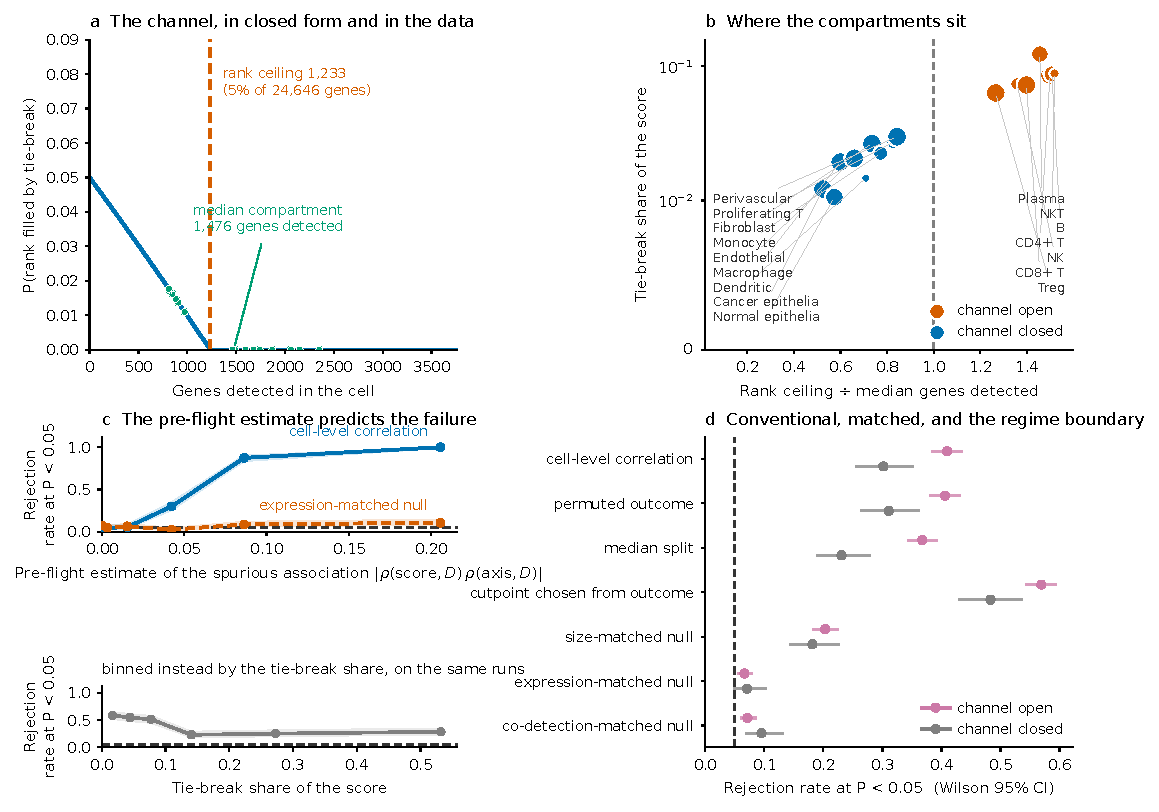
\includegraphics[width=\textwidth]{../figures/figure1_calibration.pdf}%
}{%
  \fbox{\parbox{0.9\textwidth}{\centering\vspace{2em}
  \pending\\[0.4em]
  \small Four-panel companion figure not yet rendered:
  \code{experiments/make\_figure.py} needs
  \code{results/benchmark\_gse176078\_all.csv}.
  \vspace{2em}}}%
}
\caption{\textbf{The argument in four panels.}
(\textbf{a})~Equation~\eqref{eq:channel} for the panel and ceiling of this
study, with each compartment of GSE176078 marked at its own median depth.
(\textbf{b})~The regime against what it does. The ceiling-to-depth ratio is
plotted against the share of the score that came from ranks the tie-break
settled rather than from counts the cell observed, per compartment: the x axis
is a property of the compartment's depth, the y axis is what the score did
there, and compartments to the right of the vertical line have the channel open.
(\textbf{c})~Two rows on a
shared vertical scale, both over the effect-free runs of the two calibration
sweeps: above, the rejection rate in quantile bins of \eqref{eq:implied}, for the
cell-level test and the expression-matched null; below, the same runs binned
instead by the tie-break share the paper first proposed, which falls where the
argument requires it to rise. The dashed line in
both rows is the nominal \ensuremath{\alpha = 0.05}.
(\textbf{d})~All seven analyses, split by whether there is a channel to be
confounded by.}
\label{fig:companion}
\end{figure}

\section{Reproducibility statement}
\label{sec:repro}

\paragraph{Data.} The two cohorts are public GEO series --- GSE176078
(55{,}003 cells $\times$ 24{,}646 genes; retrieved 2026-09-15) and GSE161529
(33{,}061 $\times$ 33{,}538; retrieved 2026-09-16) --- with the accession
pages linked in Data availability; gene sets are MSigDB v2024.1.Hs.
\code{results\_md5.txt} checksums every file under \code{results/}, so the
exact analysed versions are verifiable against an independent download.

\paragraph{Code.} \code{sparsegs} 0.1.0 (Python) and \code{sparseGenSetCal}
0.1.0 (R) ship with full test suites. On 2026-09-20 the Python suite passed
127 tests and the R suite passed 51 test blocks with none skipped; the
cross-language check of Methods ran clean the same day --- 216 diagnostic
reports with agreeing verdicts, 30 fixed null vectors at three tail
conventions with P values agreeing to one part in $10^{9}$, 15 pre-flights,
7 structured records identical as text, and 15 convenience calls agreeing to
one part in $10^{12}$. Environments are pinned in \code{renv.lock} (R) and
\code{environment.yml} (Python).

\paragraph{Verification.} Every rate and table is generated from the raw
JSON-line records by \code{analyse\_grid.py} and \code{make\_numbers.py}. On
2026-09-20 the generation chain was re-run over the archived records and
reproduced \code{numbers.tex} and all six generated tables byte-for-byte;
Supplementary Table~\ref{tab:verification} recomputes the headline rates
from the records independently of the generated macros, with exact agreement.

\paragraph{Records.} The five grids hold 2{,}800 records, each carrying its
seed, its realised depth statistics and every test outcome. One record,
abridged for width, reads:

\begin{verbatim}
{"grid": "A", "n_cells": 1200, "n_genes": 12000, "n_target": 8,
 "seed": 1034, "effect": 0.0, "depth_ratio": 2.094, "tie_break_share": 0.440,
 ..., "naive_reject": false, "expression_reject": false,
 "codetection_reject": false}
\end{verbatim}

\paragraph{Runtime.} The real-data benchmarks took 11{,}832~s on GSE176078
and 7{,}102~s on GSE161529 on the machine that produced them; the simulation
grids run at roughly 0.3 configurations per second on one core, so a full
regeneration of all five grids is an overnight job and parallelises across
configurations.

\paragraph{Continuous integration and archiving.} The CI workflow
(\code{.github/workflows/ci.yml}) runs on a public host on every push and is
green at the time of writing: both test suites, the cross-language check and
the offline reference check execute on a bare checkout of the repository,
the record-dependent tests skipping there by design because the records
travel with the release. The archived
release will carry a DOI (\code{XXX-DOI-XXX} pending minting). Questions
about code, data or reproducibility go to the corresponding author,
\code{duanqiwen603@gmail.com}.

\end{document}
